

\documentclass{article}

\usepackage{amsfonts, amsmath, graphicx}
\usepackage[margin=1in]{geometry}
\usepackage{natbib}
\bibliographystyle{apa-good}

\title{The Two-Foot Rule: A game theoretic analysis of the pickoff limit in Major League Baseball}

\begin{document}

  \maketitle

  \section{Introduction}
  \label{sec:introduction}

    In baseball, the stolen base is an exciting play in which a runner will take off on the pitch, attempting to reach the next base before the catcher can throw the ball to the base for a fielder to tag the runner out. Major League Baseball (MLB) stolen base totals peaked in the 1980s and 1990s but then waned in the 2000s and 2010s as teams cut back on the play, which generally requires a high success rate in order to have a positive impact on run scoring \citep{tango_book_2007}. On the micro level, it improves a team's win probability to reduce stolen base attempts that have negative expected outcomes, but on the macro level, the reduction in stolen base attempts affects the entertainment value of the game.

    Acknowledging this and other trends, MLB introduced several rule changes taking effect in the 2023 regular season, with the goal of making the game more exciting \citep{castrovince_pitch_2023}. With these changes, a pitch clock limits the time between pitches, and there are restrictions on infielder positioning, curtailing defensive shifts. Two changes are particularly relevant to stolen base attempts: Bases are now wider (reducing the distance between first and second base by 4.5 inches), and there are now count limitations on pickoff attempts, a previously unlimited deterrent of stolen bases.
    
    Whether attempting a stolen base or not, runners typically take a {\it lead} from their base, commonly positioning themselves 8--12 feet away from their base, in the direction of the next base. The longer the lead, the shorter the distance need to run on a stolen base attempt. On a pickoff attempt, instead of throwing a pitch, the pitcher will disengage from the pitching rubber and throw the ball behind the runner to a fielder covering the base, attempting to tag the runner out. Under the new rules, if the pitcher disengages from the pitching rubber three times without successfully picking off the runner, then the runner automatically advances to the next base.

    This disengagement limit creates an interesting cat-and-mouse game between the pitcher and the runner. Each unsuccessful pickoff attempt disincentivizes the pitcher from attempting another pickoff, which incentivizes the runner to increase their lead distance. But how much should the runner extend their lead? And how does the answer change depending on runner speed and other context?
    
    In the present work, we conduct the first public analysis of this game. We model the baseball inning as a Markov decision process (MDP) and solve for (a) the optimal policy for runner lead distance given current pitcher pickoff behavior and (b) the game theoretic equilibrium behavior in the two-player game between runner and pitcher. We present the practically actionable rule-of-thumb that an average runner should increase their lead distance by two feet after each disengagement.

    \subsection{Related work}

    \cite{downey_pick_2015} previously analyzed pickoff throws and stolen base attempts as a mixed strategy game without using lead distance data. They modeled the two-player game as a simultaneous decision in which the pitcher chooses whether to attempt a pickoff and the runner chooses whether to attempt a stolen base, showing that this theoretical game has a mixed-strategy Nash equilibrium. Under this equilibrium, left-handed pitchers (possessing better pickoff moves than their right-handed counterparts) would attempt fewer pickoffs and see fewer stolen bases attempted against them, a result validated by empirical data. In a later analysis, \cite{downey_pressure_2019} argued that pitchers can effectively implement a mixed strategy in low-pressure situations but struggle to randomize their decisions as pressure increases, showing a higher auto-correlation for sequential pickoff decisions in high-pressure situations. Both of these analyses covered a game in which pickoff attempts were unlimited.

    Several studies in sports economics literature have examined the extent to which professional athletes play minimax strategy. \cite{palacios-huerta_professionals_2003} found evidence consistent with minimax equilibrium behavior in the mixed strategy game of the penalty kick, in which the kicker chooses to shoot the ball left or right and the goalkeeper simultaneously chooses to dive left or right for the save. \cite{palacios-huerta_experientia_2008} followed this with a laboratory experiment featuring professional soccer players and college students simulating the penalty kick decision using cards, showing that the professionals played minimax but the students did not. On the other hand, \cite{kovash_professionals_2009} found evidence inconsistent with minimax equilibrium behavior in the National Football League (teams called more run plays and fewer pass plays than theoretically optimal) and in MLB (pitchers threw more fastballs than theoretically optimal).

    The Markov process is a very popular model in sports analytics, particularly in baseball, where the game's highly structured progression lends it well to a state space model \citep{bukiet_markov_1997}. \cite{hirotsu_using_2002} used a four-state Markov model for soccer to inform substitution decision-making based on how substitutions impact transition probabilities between states. \cite{hirotsu_markov_2003} used similar methodology to inform substitution (pinch hitting) decision-making in baseball. Recently, \cite{chan_points_2021} used a Markov model to evaluate team performance in football. More specifically, the MDP has become particularly popular model in recent years for analyzing decision-making in sports, with applications in tennis \citep{nadimpalli_when_2013}, baseball \citep{hirotsu_using_2019}, basketball \citep{sandholtz_markov_2020}, darts \citep{baird_optimising_2020} and football \citep{biro_reinforcement_2022}.

    An intermediate result of the present work is a probability model for stolen base attempts and successes (as well as an analysis how those probabilities changed with the 2023 MLB rule changes), a topic which has not received much attention. \cite{loughin_assessing_2008} estimated linear mixed-effects models for stolen base attempts and successes, using random effects for pitcher and catcher (not the runner, notably) and fixed effects for balls, strikes, outs, score, venue and pitcher hand. They showed that the spread of pitcher effects is slightly greater than the spread of catcher effects. That analysis did not have data on runner sprint speed and catcher arm strength. More recently, \cite{stanley_modeling_2023} modeled stolen base success probability using both logistic regression and a random forest, including runner sprint speed and catcher arm strength as features but excluding player identities. That analysis was limited to data prior to the 2023 MLB rule changes that incentivized base stealing.

  \section{Data}

    \subsection{MLB Stats API}
    \label{sec:statsapi}

      Most of the data used for this article were downloaded from the publicly available MLB Stats API using the R package sabRmetrics \citep{powers_sabrmetrics_2024}. The dataset comprises 722,899 plays from the 2022 MLB regular season and 726,868 plays from the 2023 MLB regular season, where each play is either a pitch or a pickoff attempt (2.0\% pickoff attempts in 2022, 1.2\% in 2023). For each play, we observe the identities of the pitcher, catcher and runners involved. Before and after each play, we observe the state of the game, described by the number of outs in the inning; which bases are occupied by runners; the ball-strike count on the batter; and the number of disengagements already used by the pitcher. On each pickoff attempt, we observe whether it is successful (runner is out) or unsuccessful (runner is safe). On each pitch, we observe whether the runner attempts a stolen base; and if so, we observe whether they are successful (runner is safe) or unsuccessful (runner is out). On each pitch terminating a plate appearance (a batting attempt by a batter), we observe the plate appearance outcome, such as strikeout, groundout, single or home run.

    \subsection{Baseball Savant}
    \label{sec:baseballsavant}

      In addition to the play-by-play data described in Section \ref{sec:statsapi}, we manually downloaded publicly available player-season level data from Baseball Savant \citep{mlb_advanced_media_notitle_2024} describing measurable performance characteristics of catchers and runners in each season, both estimated using computer vision on video data from several camera angles. For each catcher-season, we observe {\it arm strength} (miles per hour), which measures how hard the catcher throws the ball. This is defined as the average of the top 10 percent of throw speeds when the catcher is attempting to catch a base stealer. For each runner-season, we observe {\it sprint speed} (feet per second), which measures the runner's top running speed in their fastest one-second window. This is defined as the average of the top 67 percent of peak running speeds on qualified runs: (1) home-to-first runs on weakly hit batted balls and (2) runs of two or more bases on balls hit into play (excluding runs from second base on extra-base hits).

    \subsection{Proprietary Statcast Data}

      In addition to the publicly available data described in Sections \ref{sec:statsapi} and \ref{sec:baseballsavant}, this article relies on one key piece of proprietary information provided by MLB Advanced Media, estimated using computer vision on video data from several camera angles. For each play, observe each runner's {\it lead distance} (feet), which is how far they are ranging from their base at the time of the pitcher's first movement. This is defined as the distance between the runner's center of mass (projected onto the line between the runner's current base and their next base) and the nearest edge of the runner's current base. When the pitcher throws a pitch, runners will typically extend their lead by several feet from the time of the pitcher's first movement to the time of pitch release (known as taking a {\it secondary lead}), which is relevant for runner advancement on batted balls but not on stolen base attempts. Our data include only the lead distance at the time of the pitcher's first movement, not the secondary lead.

  \section{Methods}

    \subsection{Notation}

    Throughout this section, we use the following notation to describe the data observed at the beginning of each play $i \in \{1, ..., n\}$ (which can be a pitch or a pickoff attempt):
    \begin{align*}
      b_i & \in \{0, 1\}^3 \mbox{ denotes which bases (1B, 2B, 3B, respectively) are occupied;}\\
      (c_i^B, c_i^S) \equiv c_i & \in \{0, 1, 2, 3\} \times \{0, 1, 2\} \mbox{ denotes the ball-strike count;}\\
      d_i & \in \{0, 1, 2\} \mbox{ denotes the number of disengagements already used; and}\\
      o_i & \in \{0, 1, 2\} \mbox{ denotes the number of outs.}
    \end{align*}
    We use $\mathcal{H}^R$, $\mathcal{H}^P$, and $\mathcal{H}^C$ to denote the sets of runners, pitchers and catchers, respectively. On play $i$:
    \begin{align*}
      h_i^R & \in \mathcal{H}^R \mbox{ is the runner;}\\
      h_i^P & \in \mathcal{H}^P \mbox{ is the pitcher;}\\
      h_i^C & \in \mathcal{H}^C \mbox{ is the catcher;}\\
      z_i^R & \in \mathbb{R^+} \mbox{ is the sprint speed of runner $h_i^R$; and}\\
      z_i^C & \in \mathbb{R^+} \mbox{ is the arm strength of catcher $h_i^C$.}
    \end{align*}
    When the play begins, we use the following notation to describe the actions taken by the players:
    \begin{align}
    \label{eqn:runner-outcome}
      \begin{split}
        \ell_i  \in &~ \mathbb{R}^+ \mbox{ denotes the lead distance (in feet) taken by the first-base runner;}\\
        p_i \in &~ \{0, 1\} \mbox{ denotes whether the pitcher attempts (1) or does not attempt (0) a pickoff; and}\\
        r_i \in &~ \{\mbox{P}^+,\, \mbox{P}^-,\, \mbox{S}^+,\, \mbox{S}^-,\, \mbox{N}\} \equiv \mathcal{R} \mbox{ denotes the runner outcome, where}\\
          & \mbox{P}^+  \mbox{ represents a successful pickoff attempt (runner is out);}\\
          & \mbox{P}^-  \mbox{ represents an unsuccessful pickoff attempt (runner is safe);}\\
          & \mbox{S}^+  \mbox{ represents a successful stolen base attempt (runner is safe);}\\
          & \mbox{S}^-  \mbox{ represents an usuccessful stolen base attempt (runner is out); and}\\
          & \mbox{N}~   \mbox{ represents no runner action (a pitch with no stolen base attempt).}
%        p_i & \in \{0, 1\} \mbox{ indicates whether the pitcher attempts a pickoff on the first-base runner; and}\\
%        s_i & \in \{0, 1\} \mbox{ indicates whether the first-base runner attempts a stolen base.}
      \end{split}
    \end{align}
    If there is no runner on first base, then $\ell_i$ and $r_i$ are undefined.% We use a superscript to denote the success/failure of pickoff and stolen base attempts: 
%    \begin{align*}
%      p_i^+ & \in \{0, 1\} \mbox{ denotes whether the pickoff attempt is successful (i.e. the runner is tagged out); and}\\
%      s_i^+ & \in \{0, 1\} \mbox{ denotes whether the stolen base attempt is successful.}
%    \end{align*}

    \subsection{Probability model for runner outcomes}
    \label{sec:prob-runner-outcome}

      As itemized in (\ref{eqn:runner-outcome}), there are five possible outcomes for the runner with respect to the run game. To estimate each of these probabilities conditional on player identities, count and lead distance, we model four probabilities. Using $R_i$ to denote the random variable governing the probability distribution over $r_i$,
      \begin{align*}
        \pi_i    &= \mathbb{P}(R_i \in \{\mbox{P}^+,\, \mbox{P}^-\}) \mbox{ is the pickoff attempt probability;}\\
        \pi_i^+  &= \mathbb{P}(R_i \in \{\mbox{P}^+\} \mid R_i \in \{\mbox{P}^+,\, \mbox{P}^-\}) \mbox{ is the pickoff success probability;}\\
        \psi_i   &= \mathbb{P}(R_i \in \{\mbox{S}^+,\, \mbox{S}^-\} \mid R_i \in \{\mbox{S}^+,\, \mbox{S}^-, N\}) \mbox{ is the stolen base attempt probability; and}\\
        \psi_i^+ &= \mathbb{P}(R_i \in \{\mbox{S}^+\} \mid R_i \in \{\mbox{S}^+,\, \mbox{S}^-\}) \mbox{ is the stolen base success probability.}
      \end{align*}
      We estimate each of these probabilities with generalized linear mixed-effects models, implemented in R using the package lme4 \citep{bates_fitting_2015}.

      \subsubsection{Pickoff attempt probability}
      \label{sec:prob-po-attempt}

        We model $\pi_i$ using a mixed-effects logistic regression with fixed effects for balls, strikes, outs, disengagements (as a categorical), and lead distance; and with a random effect for the pitcher.
        \begin{align}
          \label{eqn:prob-po-attempt}
          \begin{split}
            \log\left(\frac{\pi_i}{1 - \pi_i}\right) &= \alpha + \beta^B c_i^B + \beta^S c_i^S + \beta^O o_i + \beta^D_{d_i} + \beta^L \ell_i + \gamma^P_{h_i^P}\\
            \gamma^P_{h} &\sim \mathcal{N}(0, \sigma^2_P) \hspace{4mm} \mbox{\it i.i.d.} \hspace{4mm} \forall h \in \mathcal{H}^P.
          \end{split}
        \end{align}
        This model has eight fixed, unknown parameters: the intercept $\alpha$; the five slopes $\beta^B$, $\beta^S$, $\beta^O$, $\beta^D$ and $\beta^L$; and the two variance parameters $\sigma^2_R$ and $\sigma^2_P$. The number of random effects is $|\mathcal{H}^R| + |\mathcal{H}^P|$.
        
      \subsubsection{Pickoff success probability}
      \label{sec:prob-po-success}

        We model $\pi_i^+$ using a mixed-effects logistic regression with a fixed effect for lead distance and a random effect for pitcher. These were the only variables for which we found substantive effects.
        \begin{align}
          \label{eqn:prob-po-success}
          \begin{split}
            \log\left(\frac{\pi_i^+}{1 - \pi_i^+}\right) &= \alpha + \beta^L \ell_i + \gamma^P_{h_i^P},\\
            \gamma^P_{h} &\sim \mathcal{N}(0, \sigma^2_P) \hspace{4mm} \mbox{\it i.i.d.} \hspace{4mm} \forall h \in \mathcal{H}^P.
          \end{split}
        \end{align}
        This model has three fixed, unknown parameters: the intercept $\alpha$, the slope $\beta^L$, and the variance parameters $\sigma^2_P$. The number of random effects is $|\mathcal{H}^P|$.

      \subsubsection{Stolen base attempt probability}
      \label{sec:prob-sb-attempt}

        Modeling the runner's decision to attempt a stolen base is complicated. One may think of this as a deterministic decision made by the runner based on the expected run value with and without attempting a steal. Such a model aligns very poorly with real decisions made by runners. We posit that the runner's ability to attempt a stolen base is influenced by external factors such as the runner's perception of the pitcher's body language timing between pitches. For this reason, we model stolen base attempts as a stochastic process rather than a deterministic decision.

        Deliberately, we exclude lead distance from the stolen base attempt model. While lead distance does help explain the probability of a stolen base attempt, this can cause problems with the framing of the runner's decision. When including lead distance, we find situations in which the expected value of a stolen base attempt is negative, and the optimal lead distance is zero feet to minimize the probability of a stolen base attempt. This is a poor reflection of reality because the runner always has the power to choose not to attempt a stolen base. We obtain a more fit-for-purpose model by excluding lead distance.

        We model $\psi_i$ using a mixed-effects logistic regression with fixed effects for balls, strikes, outs, disengagements (as a categorical), runner sprint speed, and catcher arm strength; and with random effects for runner, pitcher and catcher.
        \begin{align}
          \label{eqn:prob-sb-attempt}
          \begin{split}
            \log\left(\frac{\psi_i}{1 - \psi_i}\right) &= \alpha + \beta^B c_i^B + \beta^S c_i^S + \beta^O o_i + \beta^D_{d_i} + (\beta^R z_i^R + \gamma^R_{h_i^R}) + \gamma^P_{h_i^P} + (\beta^C z_i^C + \gamma^C_{h_i^C}),\\
            \gamma^R_{h} &\sim \mathcal{N}(0, \sigma^2_R) \hspace{4mm} \mbox{\it i.i.d.} \hspace{4mm} \forall h \in \mathcal{H}^R,\\
            \gamma^P_{h} &\sim \mathcal{N}(0, \sigma^2_P) \hspace{4mm} \mbox{\it i.i.d.} \hspace{4mm} \forall h \in \mathcal{H}^P,\\
            \gamma^C_{h} &\sim \mathcal{N}(0, \sigma^2_C) \hspace{4mm} \mbox{\it i.i.d.} \hspace{4mm} \forall h \in \mathcal{H}^C.
          \end{split}
        \end{align}
 
        We interpret $(\beta^R z_i^R + \gamma^R_{h_i^R})$ as the effect of runner $h_i^R$ on the attempt probability, combining the fixed effect of the runner's sprint speed with the random effect of their identity. By including a fixed effect for sprint speed, we are effectively regularizing the runner effects toward priors based on their sprint speeds. The interpretation of $(\beta^C z_i^C + \gamma^C_{h_i^C})$ for catchers is similar: Each catcher has an estimated effect regularized toward a prior based on their arm strength.
      
      \subsubsection{Stolen base success probability}
      \label{sec:prob-sb-success}

        We model $\psi_i^+$ using a mixed-effects logistic regression with fixed effects for lead distance, runner sprint speed, and catcher arm strength; and with random effects for runner, pitcher and catcher.
        \begin{align}
          \label{eqn:prob-sb-success}
          \begin{split}
            \log\left(\frac{\psi_i^+}{1 - \psi_i^+}\right) &= \alpha + \beta^L \ell_i + (\beta^R z_i^R + \gamma^R_{h_i^R}) + \gamma^P_{h_i^P} + (\beta^C z_i^C + \gamma^C_{h_i^C}),\\
            \gamma^R_{h} &\sim \mathcal{N}(0, \sigma^2_R) \hspace{4mm} \mbox{\it i.i.d.} \hspace{4mm} \forall h \in \mathcal{H}^R,\\
            \gamma^P_{h} &\sim \mathcal{N}(0, \sigma^2_P) \hspace{4mm} \mbox{\it i.i.d.} \hspace{4mm} \forall h \in \mathcal{H}^P,\\
            \gamma^C_{h} &\sim \mathcal{N}(0, \sigma^2_C) \hspace{4mm} \mbox{\it i.i.d.} \hspace{4mm} \forall h \in \mathcal{H}^C.
          \end{split}
        \end{align}
        As in (\ref{eqn:prob-sb-attempt}), we interpret $(\beta^R z_i^R + \gamma^R_{h_i^R})$ as the runner effect regularized toward a prior based on sprint speed and $(\beta^C z_i^C + \gamma^C_{h_i^C})$ as the catcher effect regularized toward a prior based on arm strength.

    \subsection{The baseball inning as a Markov decision process}

      \subsubsection{Markov chain model}

        Modeling the progression of a baseball inning is a well-trodden application of Markov chains in sports.(citation needed) Traditionally, the state space is defined by the bases occupied and the number of outs (24 non-terminal states, e.g., citation needed) or by those and the ball-strike count (288 non-terminal states, e.g., citation needed). To understand the game theory under the new pickoff limit rule, we take this a step further and include the number of disengagements in the state space.
      
        {\it State space.} The game state is given by $s = (b, c, d, o)$, where:
        \begin{align*}
          b &\in \{0, 1\}^3 \mbox{ represents which bases are occupied by runners};\\
          c &\in \{0, 1, 2, 3\} \times \{0, 1, 2\} \mbox{ represents the ball-strike count};\\
          d &\in \{0, 1, 2\} \mbox{ represents the number of disengagements already used}; and\\
          o &\in \{0, 1, 2\} \mbox{ represents the number of outs}.
        \end{align*}
        The total number of non-terminal states is $2^3 \times (4 \times 3) \times 3 \times 3 = 864$. There is one terminal state (end of inning), bringing the total number of states to 865. We use $\mathcal{S}$ to denote the set of all states, including the terminal state; we use $s_i = (b_i, c_i, d_i, o_i)$ to denote the starting state for play $i$; and we use $S_i$ to denote the random variable governing the probability distribution over $s_i$.
  
        {\it Transition probabilities.} The probability of transition to state $s'$ from starting state $s$ is given by the transition probability function $\mathbb{P}(S_{i+1} = s' \mid S_i = s)$. Because the present work focuses on the consequences of decisions surrounding the runner on first base, it is helpful to break down these transition probabilities by conditioning on the runner outcome:
        \begin{align}
          \label{eqn:transition-prob}
          \mathbb{P}(S_{i+1} = s' \mid S_i = s) = \sum_{r \in \mathcal{R}} \mathbb{P}(R_i = r \mid S_i = s) \cdot \mathbb{P}(S_{i+1} = s' \mid S_i = s, R_i = r).
        \end{align}

        To estimate $\mathbb{P}(R_i = r \mid S_i = s)$, we may use the empirical frequency of each runner outcome $r$ in each state $s$. In Section \ref{sec:single-agent-mdp} below, we will replace these empirical frequencies with the probabilities estimated in Section \ref{sec:prob-runner-outcome}.
        
        To estimate $\mathbb{P}(S_{i+1} = s' \mid S_i = s, R_i = r)$, we use conditional empirical frequencies of the ending state $s'$ given the starting state $s$ and the runner outcome $r$. However, we pool across the starting disengagements $d$ when calculating these empirical frequencies. Our assumption is that, given the runner event, the starting disengagements $d$ does not impact the transition probabilities between the reduced states $\tilde s \equiv (b, c, \cdot, o)$ and $\tilde s' \equiv (b', c', \cdot, o')$. By pooling data across different values of $d$, we mitigate small sample size issues when estimating transition probabilities from rare states, such as having a runner on third base with an 0-0 count, two disengagements and zero outs.
        
        The pooled empirical transition probability conditions on $e = d' - d$ instead of conditioning on $d$ and $d'$. Using $E_{i}$ to denote the random variable governing the probability distribution over $d_{i + 1} - d_i$,
        \begin{align*}
          Q(\tilde s, r, \tilde s', e)
            &= \hat{\mathbb{P}}\left(\tilde S_{i+1} = \tilde s',\, E_i = e \mid \tilde S_i = \tilde s,\, R_i = r\right)\\
            &= \frac
              {\sum_{i=1}^n\mathbb{I}\left\{\tilde s_i = \tilde s,\, r_i = r\right\} \cdot \mathbb{I}\left\{\tilde s_{i+1} = \tilde s',\, d_{i+1} - d_i = e\right\}}
              {\sum_{i=1}^n\mathbb{I}\left\{\tilde s_i = \tilde s,\, r_i = r\right\}}.
        \end{align*}
        Finally, we estimate the full-state transition probabilities as
        \begin{align*}
          \hat{\mathbb{P}}(S_{i+1} = (b', c', d', o') \mid S_i = (b, c, d, o), R_i = r) = Q\left\big((b, c, \cdot, o),\, r,\, (b', c', \cdot, o'),\, d' - d\right\big).
        \end{align*}

% NOTE (SP): I don't think we need the paragraph below, but I'm holding onto it for now in case we decide we do need it.
%        To convert the reduced-state estimated transition probabilities to full-state transition probabilities, we leverage the fact that the number of disengagements $d'$ in the ending state is a deterministic function of the starting disengagements $d$, the runner outcome $r$ and  the ending count $c'$:
%        \begin{align}
%          \label{eqn:disengagement-transition}
%          d' = D(d, c', r)
%            \equiv \begin{cases}
%            \hfil d & \mbox{if } r \in \{\mbox{N}\} \mbox{ and } c' \ne (0, 0)\\
%            \hfil 0 & \mbox{if } r \in \{\mbox{N}\} \mbox{ and } c' = (0, 0)\\
%            d + 1   & \mbox{if } r \in \{\mbox{P}^-\} \mbox{ and } d < 2\\
%            \hfil 0 & \mbox{if } r \in \{\mbox{P}^-\} \mbox{ and } d = 2\\
%            \hfil 0 & \mbox{if } r \in \{\mbox{P}^+,\, \mbox{S}^+,\, \mbox{S}^-\}\\
%          \end{cases}.
%        \end{align}
 
      \subsubsection{Single-agent Markov decision process}
      \label{sec:single-agent-mdp}

        The MDP is an extension of the Markov chain model that allows for deterministic actions which change transition probabilities between states. In this section we allow for the runner to choose a lead distance $\ell$, and we model the pitcher's decision whether to attempt a pickoff as a stochastic process (see Section \ref{sec:prob-po-attempt}). We call this the {\it single-agent} model because only the runner has agency in this model of the game. We limit this action to states in which first base is occupied and the other bases are unoccupied, i.e. $b = (1, 0, 0)$. This limits our scope to situations in which the runner might steal second base (encompassing XX\%\footnote{TODO: fill this in} of stolen base attempts in 2023) and excludes the first-and-third scenario $b = (1, 0, 1)$, in which the first-base runner will often attempt a stolen base to lure a throw from the catcher, giving the third-base runner a chance to steal home.
     
        {\it Action space.} In states for which $b = (1, 0, 0)$, the first-base runner must choose a lead distance $\ell \in [0, 20] \equiv \mathcal{L}$, representing distance in feet from first base. For computational purposes, we discretize this action space by rounding $\ell$ to the nearest tenth of a foot, meaning that there are 201 possible actions.
  
        {\it Transition probabilities.} The probability of transition to ending state $s'$ from starting state $s$ given lead distance $\ell$ is $P(s' \mid s,\, \ell) = \mathbb{P}(S_{i+1} = s' \mid S_i = s,\, \ell_i = \ell)$. To estimate state transition probabilities that depend on lead distance, we modify (\ref{eqn:transition-prob}) by conditioning on the lead distance:
        \begin{align}
          \label{eqn:transition-prob-lead}
          P(s' \mid s,\, \ell) = \sum_{r \in \mathcal{R}} \mathbb{P}(R_i = r \mid S_i = s,\, \ell_i = \ell) \cdot \mathbb{P}(S_{i+1} = s' \mid S_i = s,\, R_i = r).
        \end{align}
        In this equation, the runner outcome depends on the lead distance, but we assume that given the runner outcome, the state transition is independent of the lead distance. The procedure for estimating $\mathbb{P}(S_{i+1} = s' \mid S_i = s,\, R_i = r)$ is described in Section \ref{sec:single-agent-mdp}. To estimate $\mathbb{P}(R_i = r \mid S_i = s,\, \ell_i = \ell)$, we use the models from Section \ref{sec:prob-runner-outcome}. Specifically, $\mathbb{P}(R_i = r \mid S_i = s,\, \ell_i = \ell,\, p_i = p)$ is given by
        \begin{align*}
          \begin{cases}
              \hfil \pi_i(\ell) \cdot \pi_i^+(\ell)                             & \mbox{if } r = \mbox{P}^+\\
              \hfil \pi_i(\ell) \cdot (1 - \pi_i^+(\ell))                       & \mbox{if } r = \mbox{P}^-\\
              \hfil (1 - \pi_i(\ell)) \cdot \psi_i \cdot \psi_i^+(\ell)         & \mbox{if } r = \mbox{S}^+\\
              \hfil (1 - \pi_i(\ell)) \cdot \psi_i \cdot (1 - \psi_i^+(\ell))   & \mbox{if } r = \mbox{S}^-\\
              \hfil (1 - \pi_i(\ell)) \cdot (1 - \psi_i)                        & \mbox{if } r = \mbox{N}\\
          \end{cases}.
        \end{align*}
        Recall that the stolen base attempt probability $\psi_i$ does not depend on $\ell$, as described in Section \ref{eqn:prob-sb-attempt}.
  
        {\it Reward function.} The reward function for transitioning from state $s$ to state $s'$ is given by the number of runs scored in the transition. Note that this reward function does not depend on the action taken by the runner, so we can write $R(s, \ell, s') = R(s, s')$. If $s = (b, c, d, o)$ and $s' = (b', c', d', o')$, then:
        \begin{align}
          \label{eqn:reward}
          R(s, s') = (g(b') + o') - (g(b) + o) - \mathbb{I}\{c' = (0, 0),\, d' = 0\},
        \end{align}
        where $g: \{0, 1\}^3 \rightarrow \{0, 1, 2, 3\}$ counts the number of runners on base. This expression for the reward function counts the total number of baserunners and outs before and after the transition and subtracts one if the transition corresponds to the end of a plate appearance. For transitions to the terminal end-of-inning state, the number of runs scored may not be uniquely determined by the starting state. To handle this case, we introduce intermediary states which track the number of runs scored on the last play, only for transitions to the terminal end-of-inning state. These intermediary states transition to the terminal end-of-inning state with probability 1.

        {\it Policy iteration.} A policy function $\pi : \mathcal{S} \rightarrow \mathcal{L}$ maps the state space to the action space, defining the lead distance to be taken by the runner in each state. The policy function $\pi$ specifies transition probabilities $P(s' \mid s,\, \ell = \pi(s))$ and induces a probability distribution over the sequence of states $\{S_t\}_{t=1}^\infty$. The value function $V_\pi : \mathcal{S} \rightarrow \mathbb{R}^+$ is the expected sum of rewards with respect to this probability distribution, which we interpret as the expected number of runs scored in the inning, starting from state $s$:
        \begin{align}
          \label{eqn:run-expectancy}
          V_\pi(s) = \mathbb{E}_\pi\left[\left.\sum_{t = 0}^\infty R(S_{t}, S_{t+1})~\right|~S_0 = s\right].
        \end{align}
        
        The relevant question for the runner is, ``What lead distance should I choose in each situation to maximize run scoring overall?'' We find the policy function $\pi^*$ which maximizes (\ref{eqn:run-expectancy}) via policy iteration (citation needed) by initializing $\hat V_0(s) = 0$ and $\hat \pi_0(s) = 0$ for all $s \in \mathcal{S}$, and then iteratively applying the updates
        \begin{align}
          \label{eqn:update-value-single-agent}
          \hat V_{i+1}(s) &= \sum_{s' \in \mathcal{S}} P(s' | s,\, \hat\pi_i(s)) [R(s, s') + \hat V_i(s')] && \forall s \in \mathcal{S}, \mbox{ and}\\
          \label{eqn:update-policy-single-agent}
          \hat\pi_{i+1}(s) &= \arg\max_{\ell \in \mathcal{L}} \sum_{s' \in \mathcal{S}} P(s' | s,\, \ell) [R(s, s') + \hat V_{i+1}(s')] && \forall s \in \mathcal{S},
        \end{align}
        until $\max_{s\in\mathcal{S}}|\pi_{i+1}(s) - \pi_i(s)|$ converges to zero.\footnote{Are we guaranteed convergence? Are we guaranteed convergence to the optimal policy?}
    
      \subsubsection{Two-agent Markov decision process}
      \label{sec:two-agent-mdp}

        In this section we extend the single-agent model by allowing the pitcher to choose whether to attempt a pickoff. We call this the {\it two-agent} model because both the runner and the pitcher have agency in this model of the game. Specifically, we model this as a two-stage game, where the runner first chooses a lead distance, and then the pitcher decides whether to attempt a pickoff after observing the runner's lead distance.

        {\it Action space.} As in the single-agent model, we limit actions to states in which only first base is occupied. The runner chooses a lead distance $\ell \in \mathcal{L}$, and then the pitcher chooses a pickoff action $p \in \{0, 1\} \equiv \mathcal{P}$, where $p = 1$ corresponds to a pickoff attempt.

        {\it Transition probabilities.} The probability of transition to ending state $s'$ from starting state $s$ given lead distance $\ell$ and pickoff decision $p$ is $P(s' \mid s,\, \ell,\, p) = \mathbb{P}(S_{i+1} = s' \mid S_i = s,\, \ell_i = \ell,\, p_i = p)$. We modify (\ref{eqn:transition-prob-lead}) by conditioning additionally on the pickoff decision:
        \begin{align}
          \label{eqn:transition-prob-lead-pickoff}
          P(s' \mid s, \ell, p) = \sum_{r \in \mathcal{R}} \mathbb{P}(R_i = r \mid S_i = s,\, \ell_i = \ell,\, p_i = p) \cdot \mathbb{P}(S_{i+1} = s' \mid S_i = s,\, R_i = r),
        \end{align}
        where $\mathbb{P}(R_i = r \mid S_i = s,\, \ell_i = \ell,\, p_i = p)$ is given by
        \begin{align*}
            \begin{cases}
                \hfil p \cdot \pi_i^+(\ell)                             & \mbox{if } r = \mbox{P}^+\\
                \hfil p \cdot (1 - \pi_i^+(\ell))                       & \mbox{if } r = \mbox{P}^-\\
                \hfil (1 - p) \cdot \psi_i \cdot \psi_i^+(\ell)         & \mbox{if } r = \mbox{S}^+\\
                \hfil (1 - p) \cdot \psi_i \cdot (1 - \psi_i^+(\ell))   & \mbox{if } r = \mbox{S}^-\\
                \hfil (1 - p) \cdot (1 - \psi_i)                        & \mbox{if } r = \mbox{N}\\
            \end{cases}.
        \end{align*}

        {\it Reward function.} The reward function (\ref{eqn:reward}) is the same for the two-agent model as for the single-agent model. In this game, however, the runner wants to maximize the reward, and the pitcher wants to minimize the reward.

        {\it Policy iteration.} In the policy update step (\ref{eqn:update-policy-single-agent}) of policy iteration for the single-agent model, we seek the policy which maximizes the expected one-step sum of reward and resulting value, given an estimated value function. In the two-agent model, there are game theoretic considerations. Given the estimated value function $\hat V$ and the runner's chosen lead distance $\ell$, the pitcher chooses $p$ to minimize the expected one-step sum of reward and resulting value:
        \begin{align*}
          \arg\min_{p\in\mathcal{P}} \sum_{s' \in \mathcal{S}} P(s' \mid s,\, \ell,\, p) [R(s, s') + \hat V(s')].
        \end{align*}
        Knowing that this is the optimal behavior for the pitcher, the runner chooses their lead distance to maximize the resulting run value:
        \begin{align*}
          \arg\max_{\ell \in \mathcal{L}}\left\{\min_{p\in\mathcal{P}} \sum_{s' \in \mathcal{S}} P(s' \mid s,\, \ell,\, p) [R(s, s') + \hat V(s')]\right\}.
        \end{align*}

        The optimal policy for the pitcher is clear: between the choices of attempting a pickoff or not, make the choice that results in the lower run expectation. To find the optimal policy $\pi^* : \mathcal{S} \rightarrow \mathcal{L}$ for the runner, we again apply policy iteration. Starting with $\hat V_0(s) = 0$ and $\hat \pi_0(s) = 0$ for all $s \in \mathcal{S}$, we iteratively apply the updates below until the policy converges.\footnote{TODO: Are we guaranteed convergence to the optimal policy?}
        
        \begin{align}
          \label{eqn:update-value-two-agent}
          \hat V_{i+1}(s) &= \min_{p \in \mathcal{P}} \sum_{s' \in \mathcal{S}} P(s' | s,\, \hat\pi_i(s)) [R(s, s') + \hat V_i(s')] && \forall s \in \mathcal{S}, \mbox{ and}\\
          \label{eqn:update-policy-two-agent}
          \hat\pi_{i+1}(s) &= \arg\max_{\ell \in \mathcal{L}} \left\{\min_{p \in \mathcal{P}}\sum_{s' \in \mathcal{S}} P(s' | s,\, \ell,\, p) [R(s, s') + \hat V_{i+1}(s')]\right\} && \forall s \in \mathcal{S}.
        \end{align}

        Given this runner policy, the pitcher is indifferent between throwing a pitch and attempting a pickoff.

  \section{Results}
  
    \subsection{Observed runner behavior}

      As detailed in Section \ref{sec:introduction}, MLB made several rule changes between the 2022 season and the 2023 season, most notably (for the present work) widening the bases and limiting the number of pickoffs that can be attempted by the pitcher. Figure \ref{fig:leads-overall} illustrates the difference in runner lead distance behavior (from first base) between 2022 and 2023. With zero disengagements in 2023, the distribution of lead distances is very similar to the overall distribution of lead distances in 2022. With each successive disengagement, we observe a positive shift in the distribution of lead distance in the 2023 data. In 2022, the average lead distance was XX feet. In 2023, the average lead distance under 0, 1 and 2 disengagements was XX feet, XX feet and XX feet, respectively.
 
      \begin{figure}
        \centering
        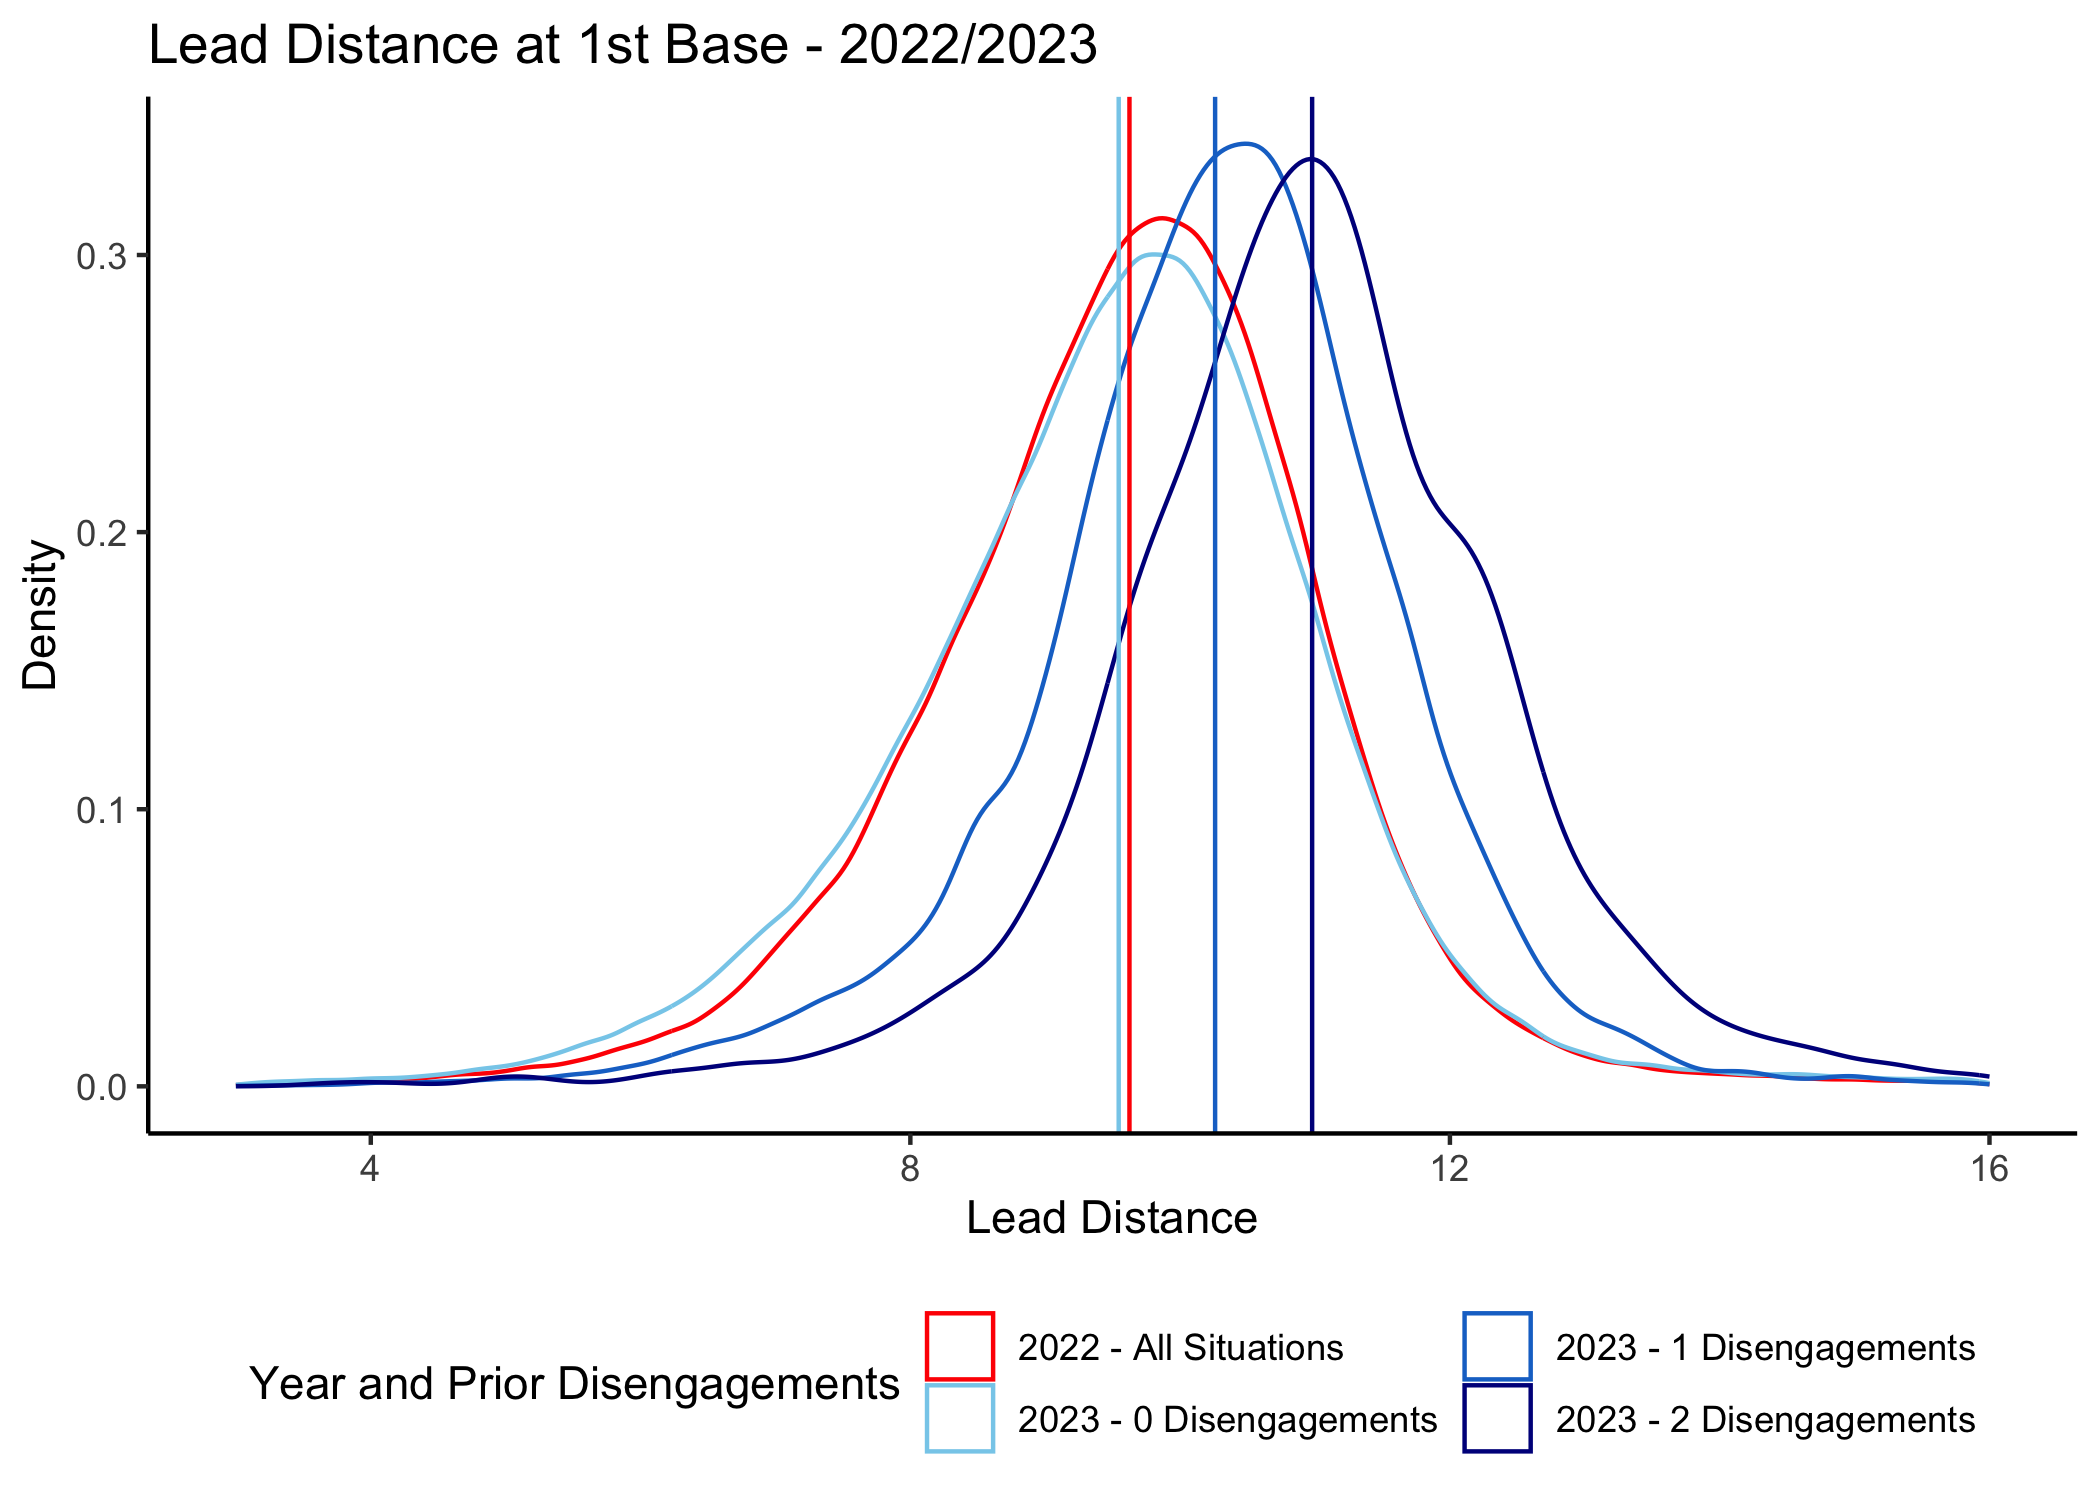
\includegraphics[width = 0.8\textwidth]{figures/leads_overall.png}
        \caption{
          \it The league-wide distribution of lead distance from first base when second base is unoccupied, comparing 2022 with 2023. The 2023 data are split by prior disengagements because, beginning in 2023, pitchers were limited to three disengagements, influencing pitcher and runner behavior. In 2022, there was no limit on the number of disengagements. The vertical lines mark the means of the distributions.
        }
        \label{fig:leads-overall}
      \end{figure}
      
    \subsection{Probability model for runner outcomes}

      Figures \ref{fig:prob-pickoff-attempt}-\ref{fig:prob-sb-success} illustrate the relationship between lead distance and runner outcome probabilities, as estimated using the mixed-effects logistic regression models detailed in Section \ref{sec:prob-runner-outcome}. For all three models, the direction of the relationship between lead distance and outcome probability is as expected.

      Figure \ref{fig:prob-pickoff-attempt} shows pickoff attempt probability modeled as a function of lead distance, split by season and number of prior disengagements. We observe that pickoff attempt rates were lower in 2023 than in 2022, especially as the number of prior disengagement increased. The modeled probability remains low even for extremely long leads, such as 20 feet. We have very limited data on lead distances beyond 14 feet, especially with fewer than two prior disengagements, so extrapolation much beyond 14 feet is likely not reliable. The ball-strike count and the identity of the pitcher also influence the pickoff attempt probability, but the primary drivers are lead distance and the number prior disengagements.
      
      \begin{figure}
        \centering
        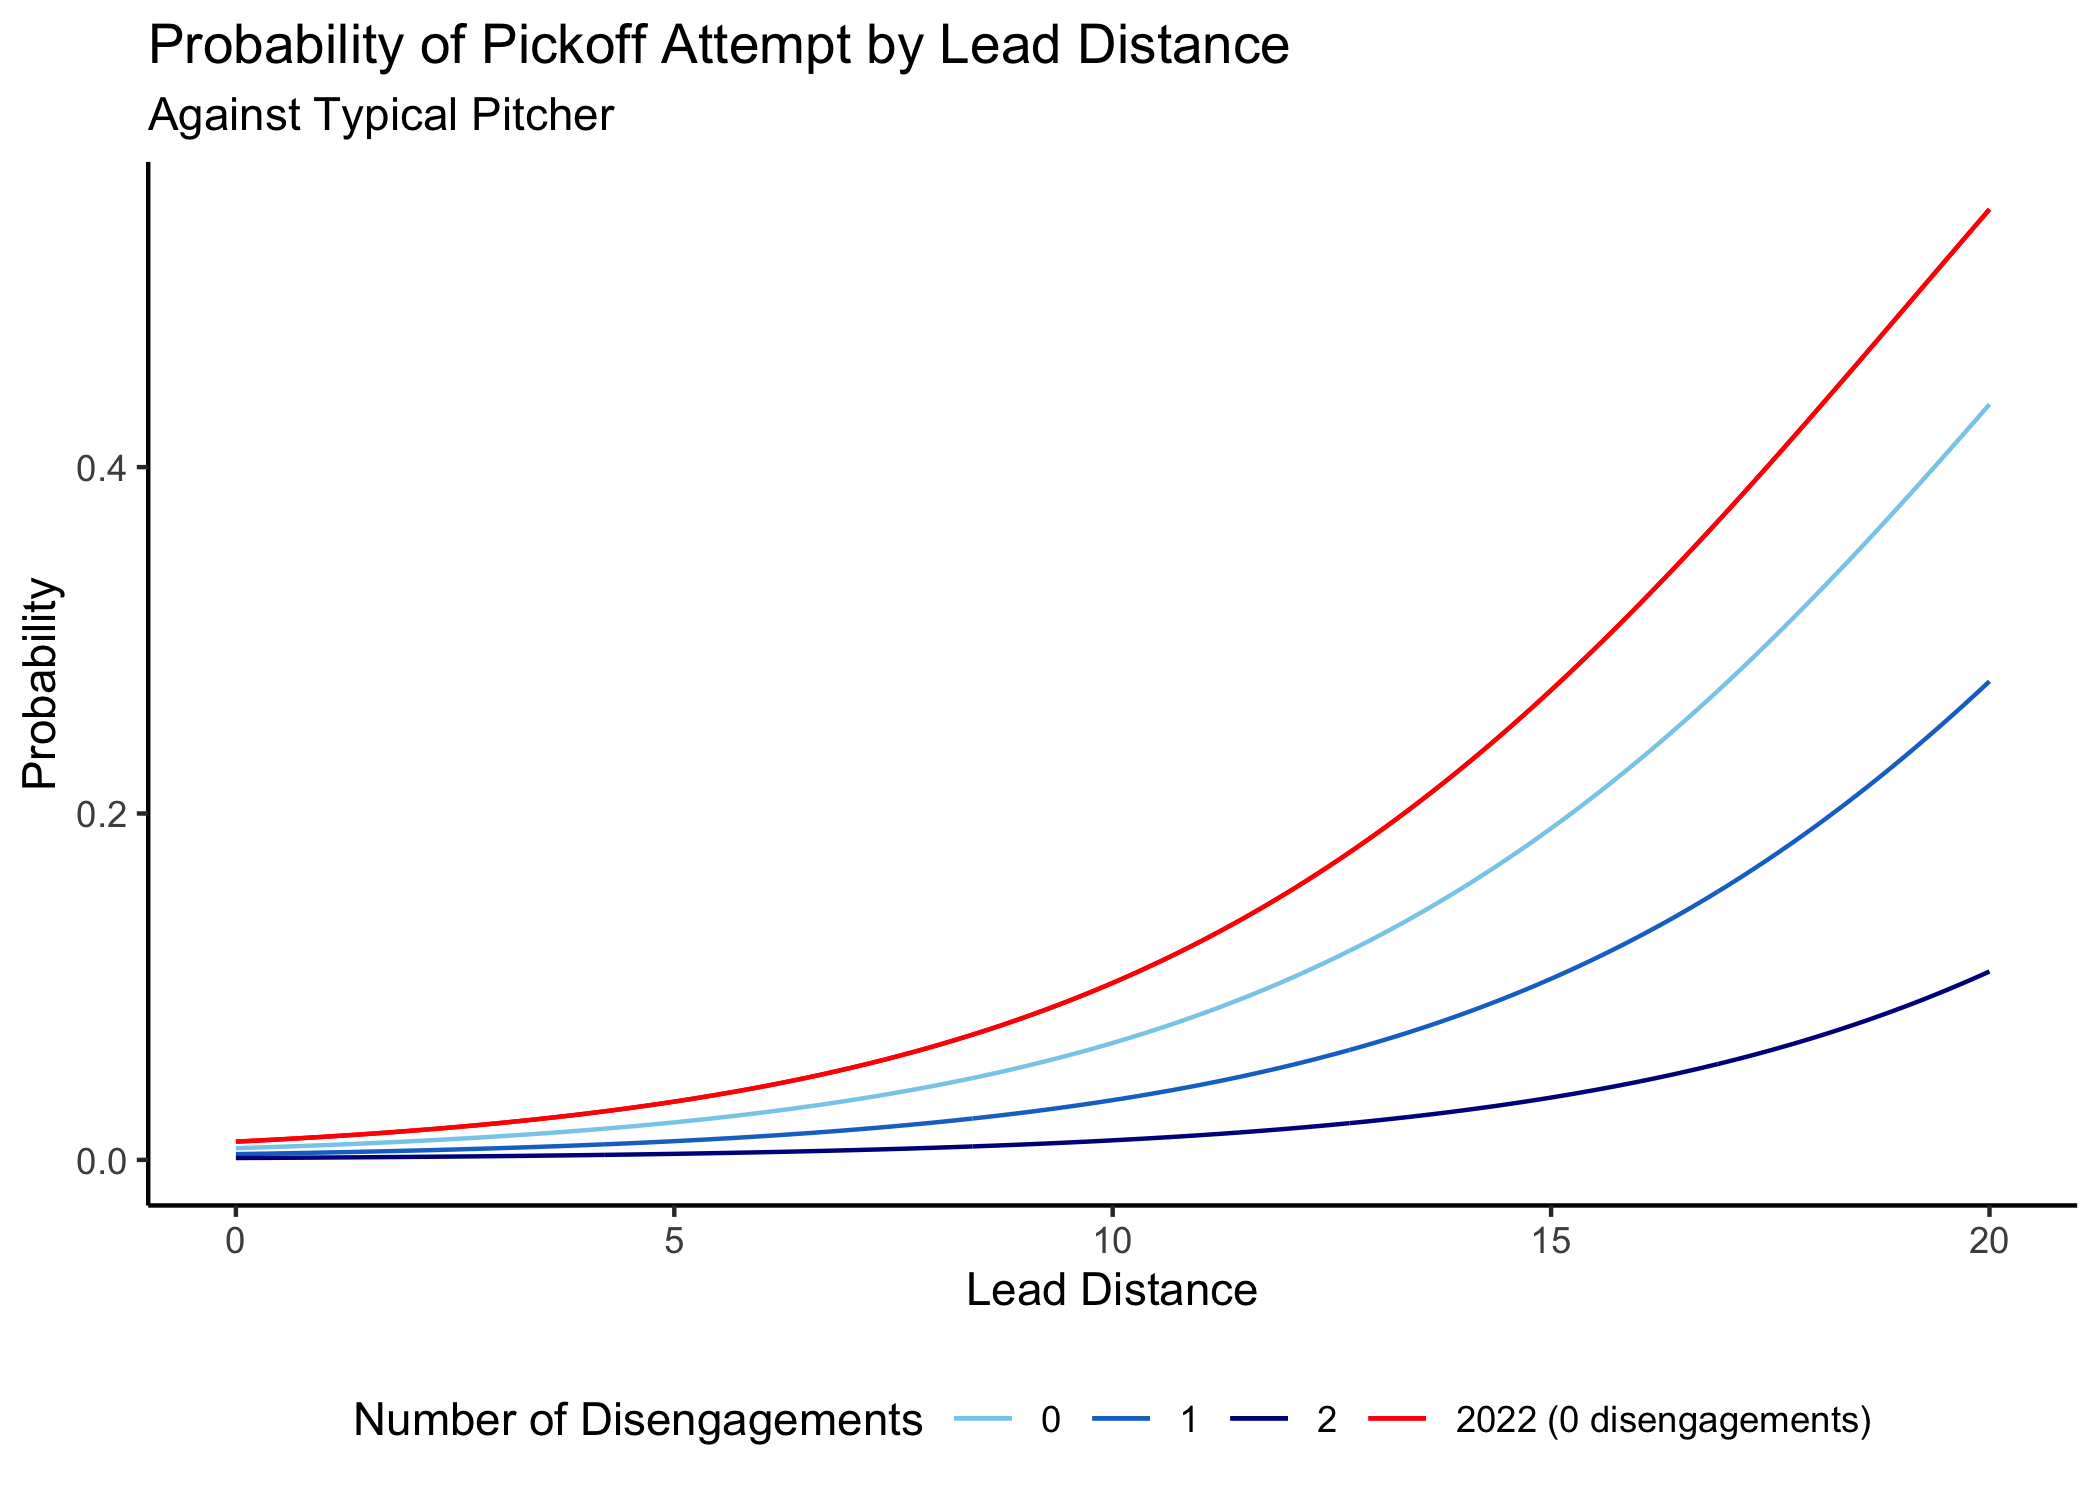
\includegraphics[width = 0.8\textwidth]{figures/prob_pickoff_attempt.png}
        \caption{
          \it Pickoff attempt probability modeled as function of lead distance, split by season and number of prior disengagements. This figure shows the probability estimated by the model detailed in Section \ref{sec:prob-po-attempt}, assuming 0 balls, 0 strikes, 0 outs and a median pitcher random effect.
        }
        \label{fig:prob-pickoff-attempt}
      \end{figure}
      
      Figure \ref{fig:prob-pickoff-success} shows pickoff success probability modeled as a function of lead distance, split by pitcher pickoff skill (based on their random effect from the mixed-effect logistic regression). We observe that, except for the most skilled pitchers, pickoff attempt probability is very low within the range covering the vast majority of lead distances. Toward the high end of this range, the success rate increases quickly as lead distance increases. Interestingly, there is a large gap between the 90$^{th}$-percentile pitcher and the median pitcher but a small gap between the median pitcher and the 10$^{th}$-percentile pitcher, demonstrating a right skew in the distribution of pitcher pickoff skill. Earlier exploration indicated that game state and runner identity did not provide predictive value for pickoff success given lead distance.
  
      \begin{figure}
        \centering
        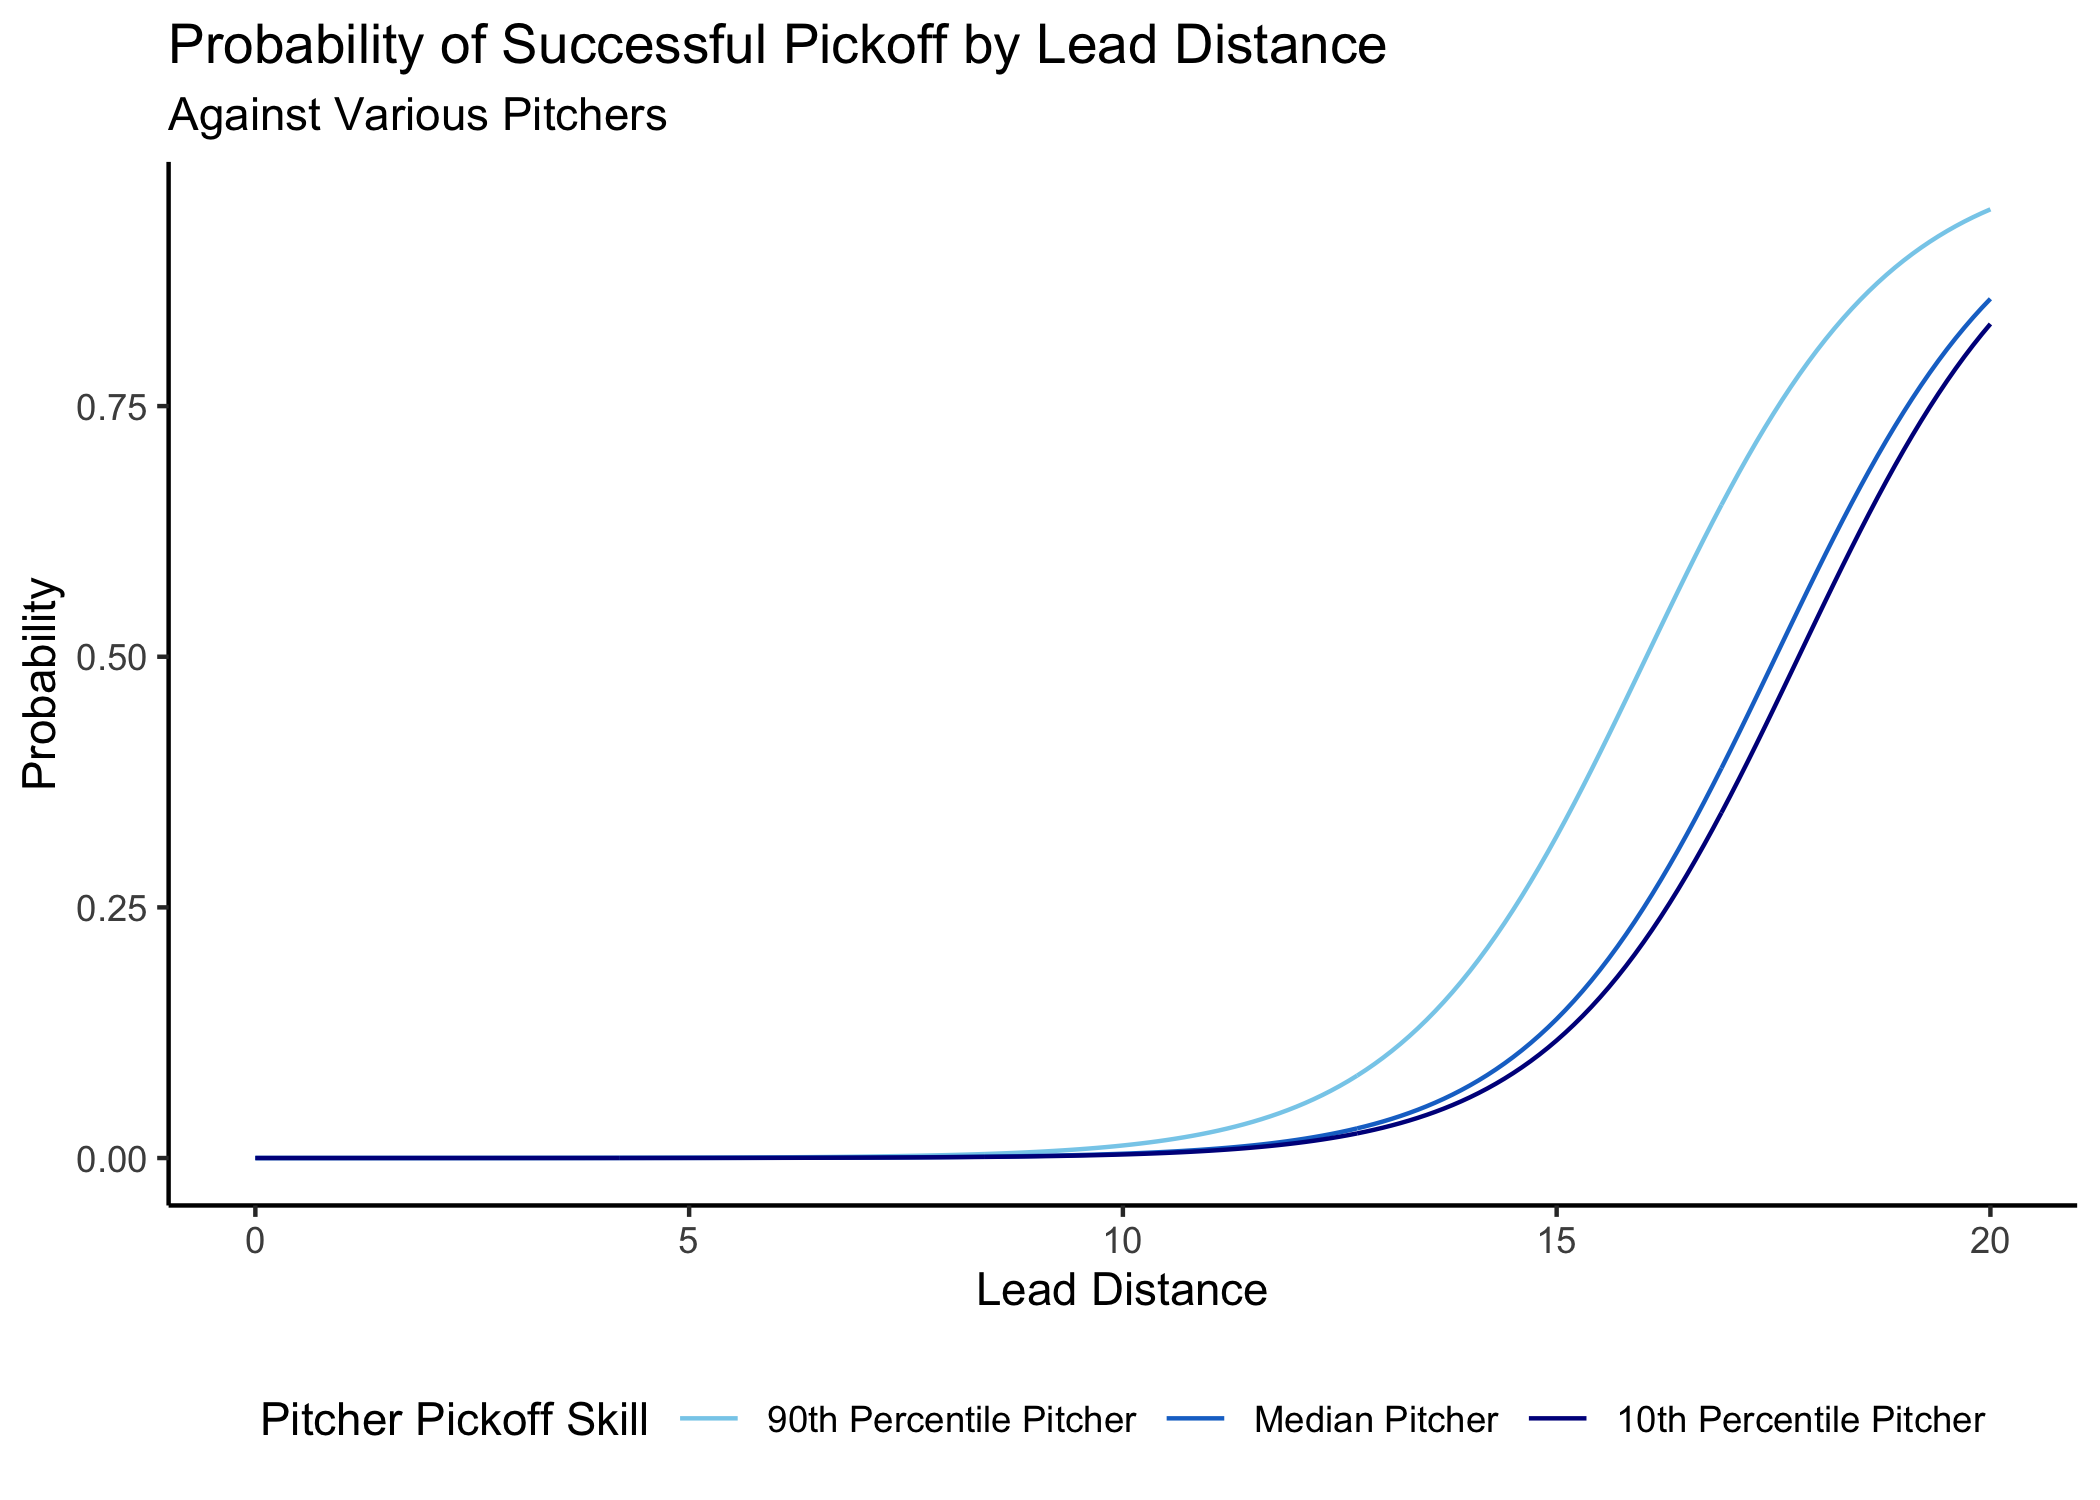
\includegraphics[width = 0.8\textwidth]{figures/prob_pickoff_success.png}
        \caption{
          \it Pickoff success probability modeled as function of lead distance, split by pitcher random effect. This figure shows the probability estimated by the model detailed in Section \ref{sec:prob-po-success}, which includes only an intercept, a fixed effect for lead distance and a random effect for pitcher identity.
        }
        \label{fig:prob-pickoff-success}
      \end{figure}

      The stolen base attempt probability model does not include lead distance, as explained in Section \ref{sec:prob-sb-attempt}. As a result, this model has only a secondary effect on the lead distance policies learned in later sections.

      Figure \ref{fig:prob-sb-success} shows stolen base success probability modeled as function of lead distance, split by season and by runner skill (based on sprint speed and runner random effect). We observe that, conditioned on lead distance, even 10$^{th}$-percentile runners in 2023 outperformed the median runner in 2022, which is likely attributable to rule changes making it easier to successfully steal bases in 2023. Within the range covering most lead distances, the difference between the 90$^{th}$-percentile runner and the median runner is just under 5 percentage points of success probability, similar to the difference between the median runner and the 10$^{th}$-percentile runner. Base-out state and {\it battery} (i.e. pitcher and catcher) skill also influence stolen base success probability although they are not shown in this visualization.
      
      \begin{figure}
        \centering
        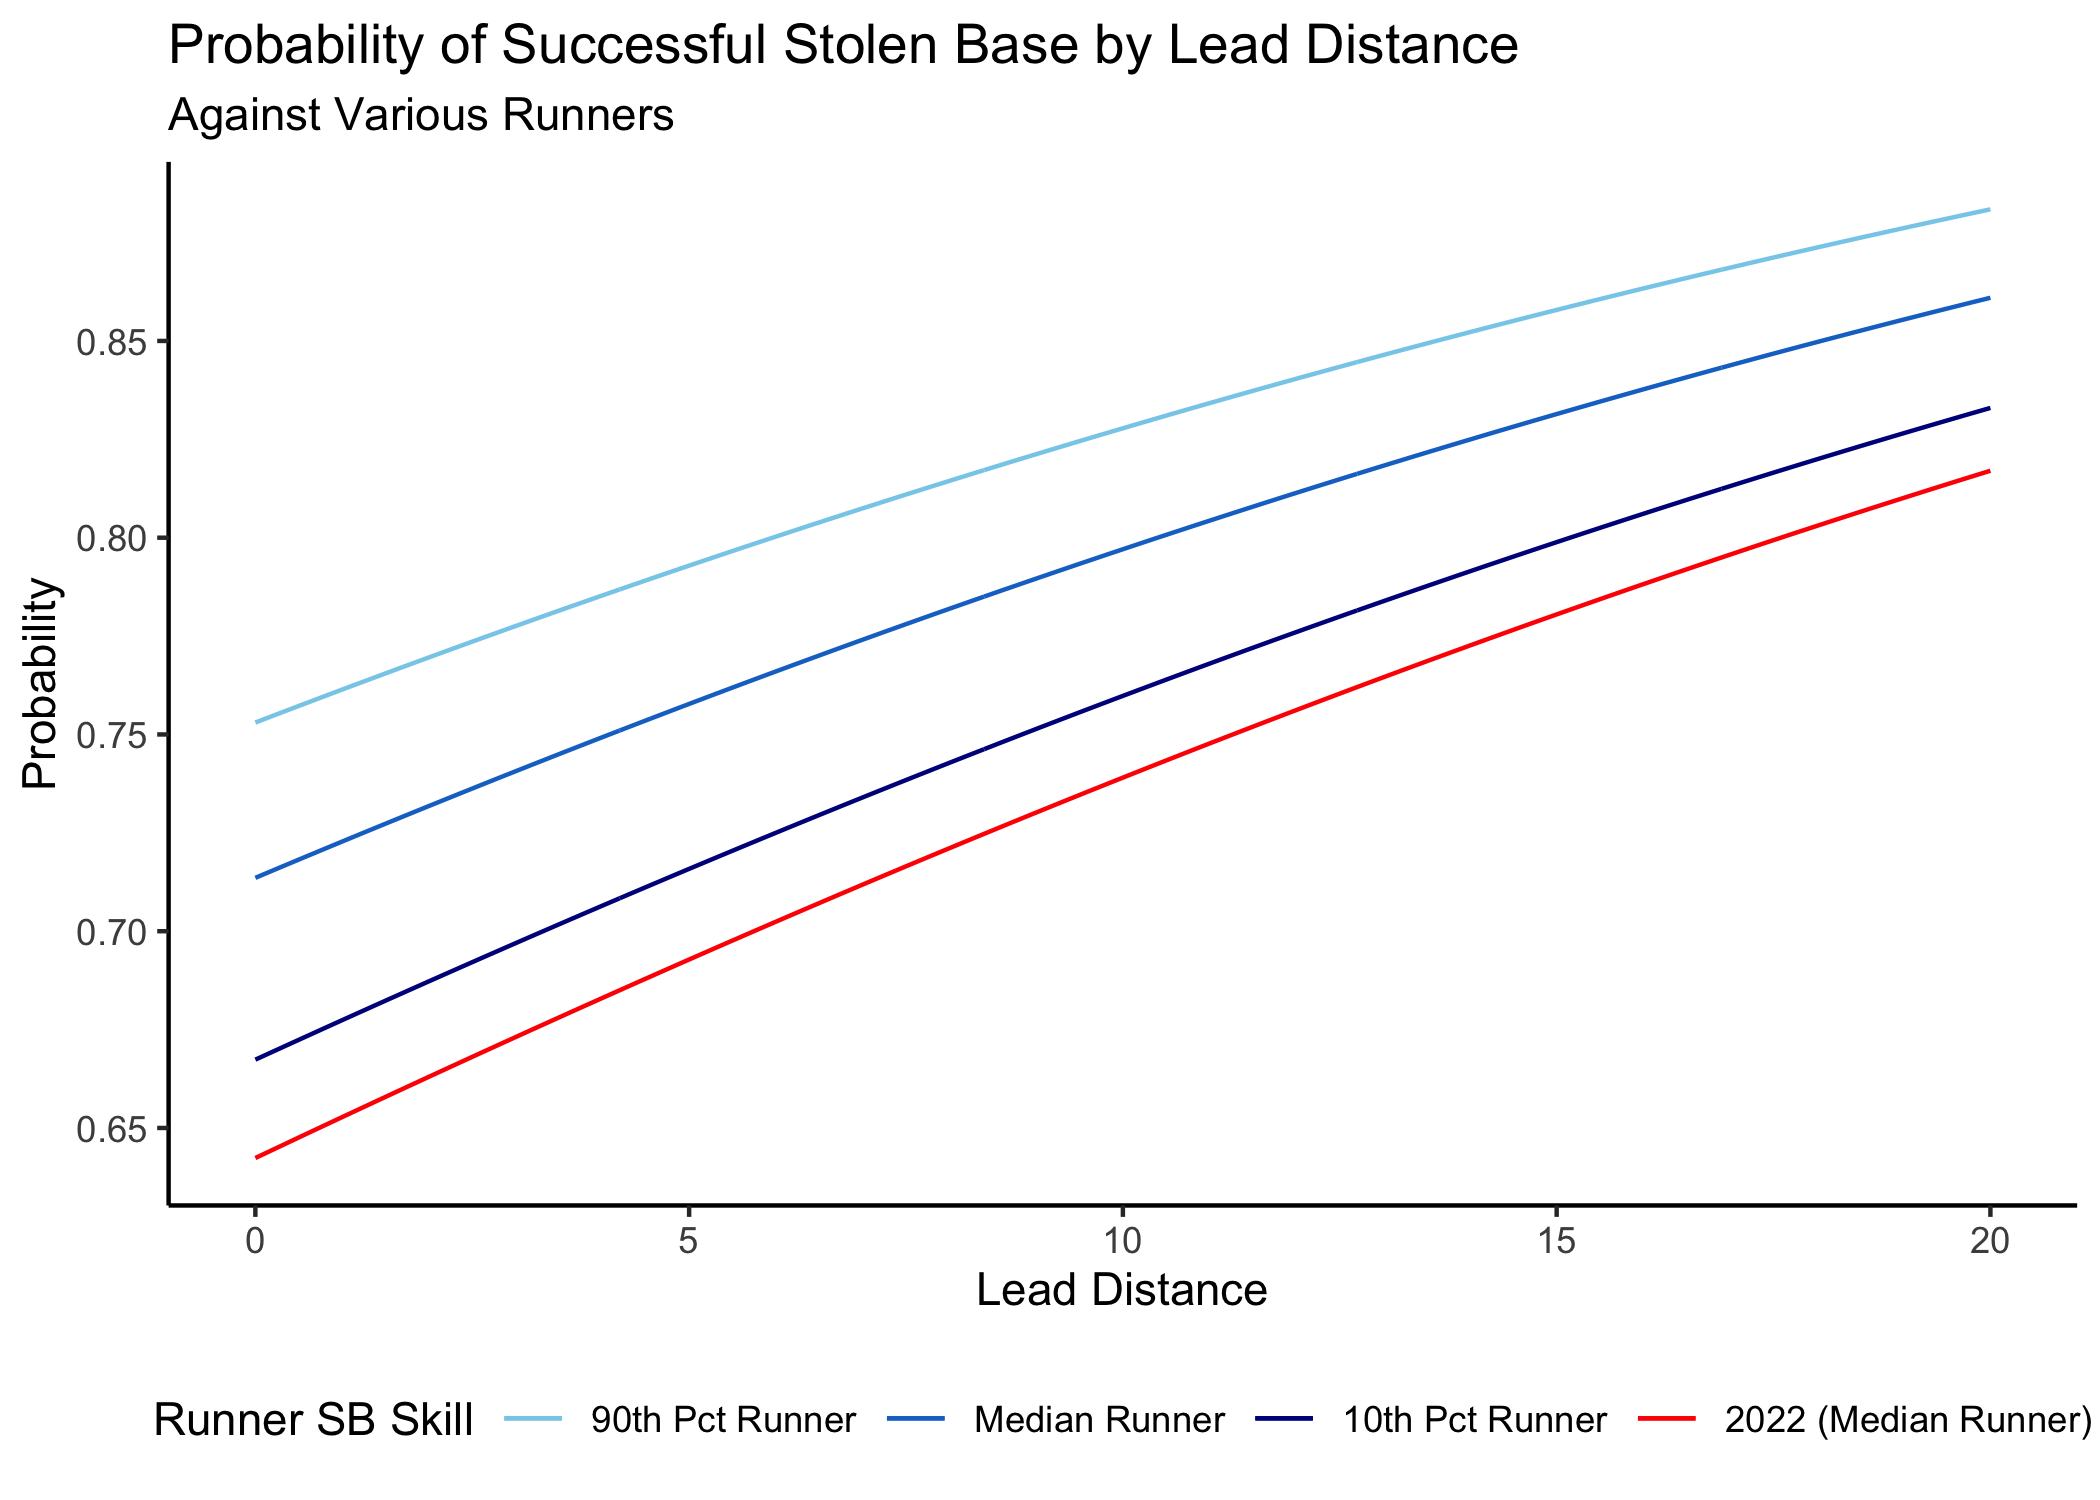
\includegraphics[width = 0.8\textwidth]{figures/prob_sb_success.png}
        \caption{
          \it Stolen base success probability modeled as function of lead distance, split by season and runner effect (combining the fixed effect of runner sprint speed and the random effect of runner identity). This figure shows the probability estimated by the model detailed in Section \ref{sec:prob-sb-success}, assuming 0 balls, 0 strikes, 0 outs and a median value for the combined effect of pitcher identity (random effect), catcher arm strength (fixed effect) and catcher identity (random effect).
        }
        \label{fig:prob-sb-success}
      \end{figure}

      A novel aspect of these runner outcome probability models is the combination of fixed effects for measurable player characteristics (catcher arm strength and runner sprint speed). This feature allows us to answer questions such as: How important are these measurable characteristics for player performance outcomes? And to what extent do players over- or under-perform what is expected from their measurable characteristics? The combination of the fixed effect and the random effect gives us an estimate (which we call the {\it combined effect}) of each player's skill, regularized toward what is expected from their measurable characteristics.

      For the stolen base success probability model, Figure \ref{fig:random-effect} shows the relationship between the combined player effect and the corresponding measurable characteristic, for both catchers and runners. We observe that arm strength explains 65\% of the variance in the catcher combined effect and that sprint speed explains 86\% of the variance in the runner combined effect. In other words, sprint speed tells us more about runner skill than arm strength tells us about catcher skill, with regard to stolen base outcomes. Beyond arm strength, the catcher can reduce stolen base success by releasing the ball more quickly or by throwing it more accurately to the target base. Beyond sprint speed, the runner can increase stolen base success by starting to run earlier (i.e., getting a better jump) or by accelerating more quickly to their top speed.
      
      \begin{figure}
        \centering
        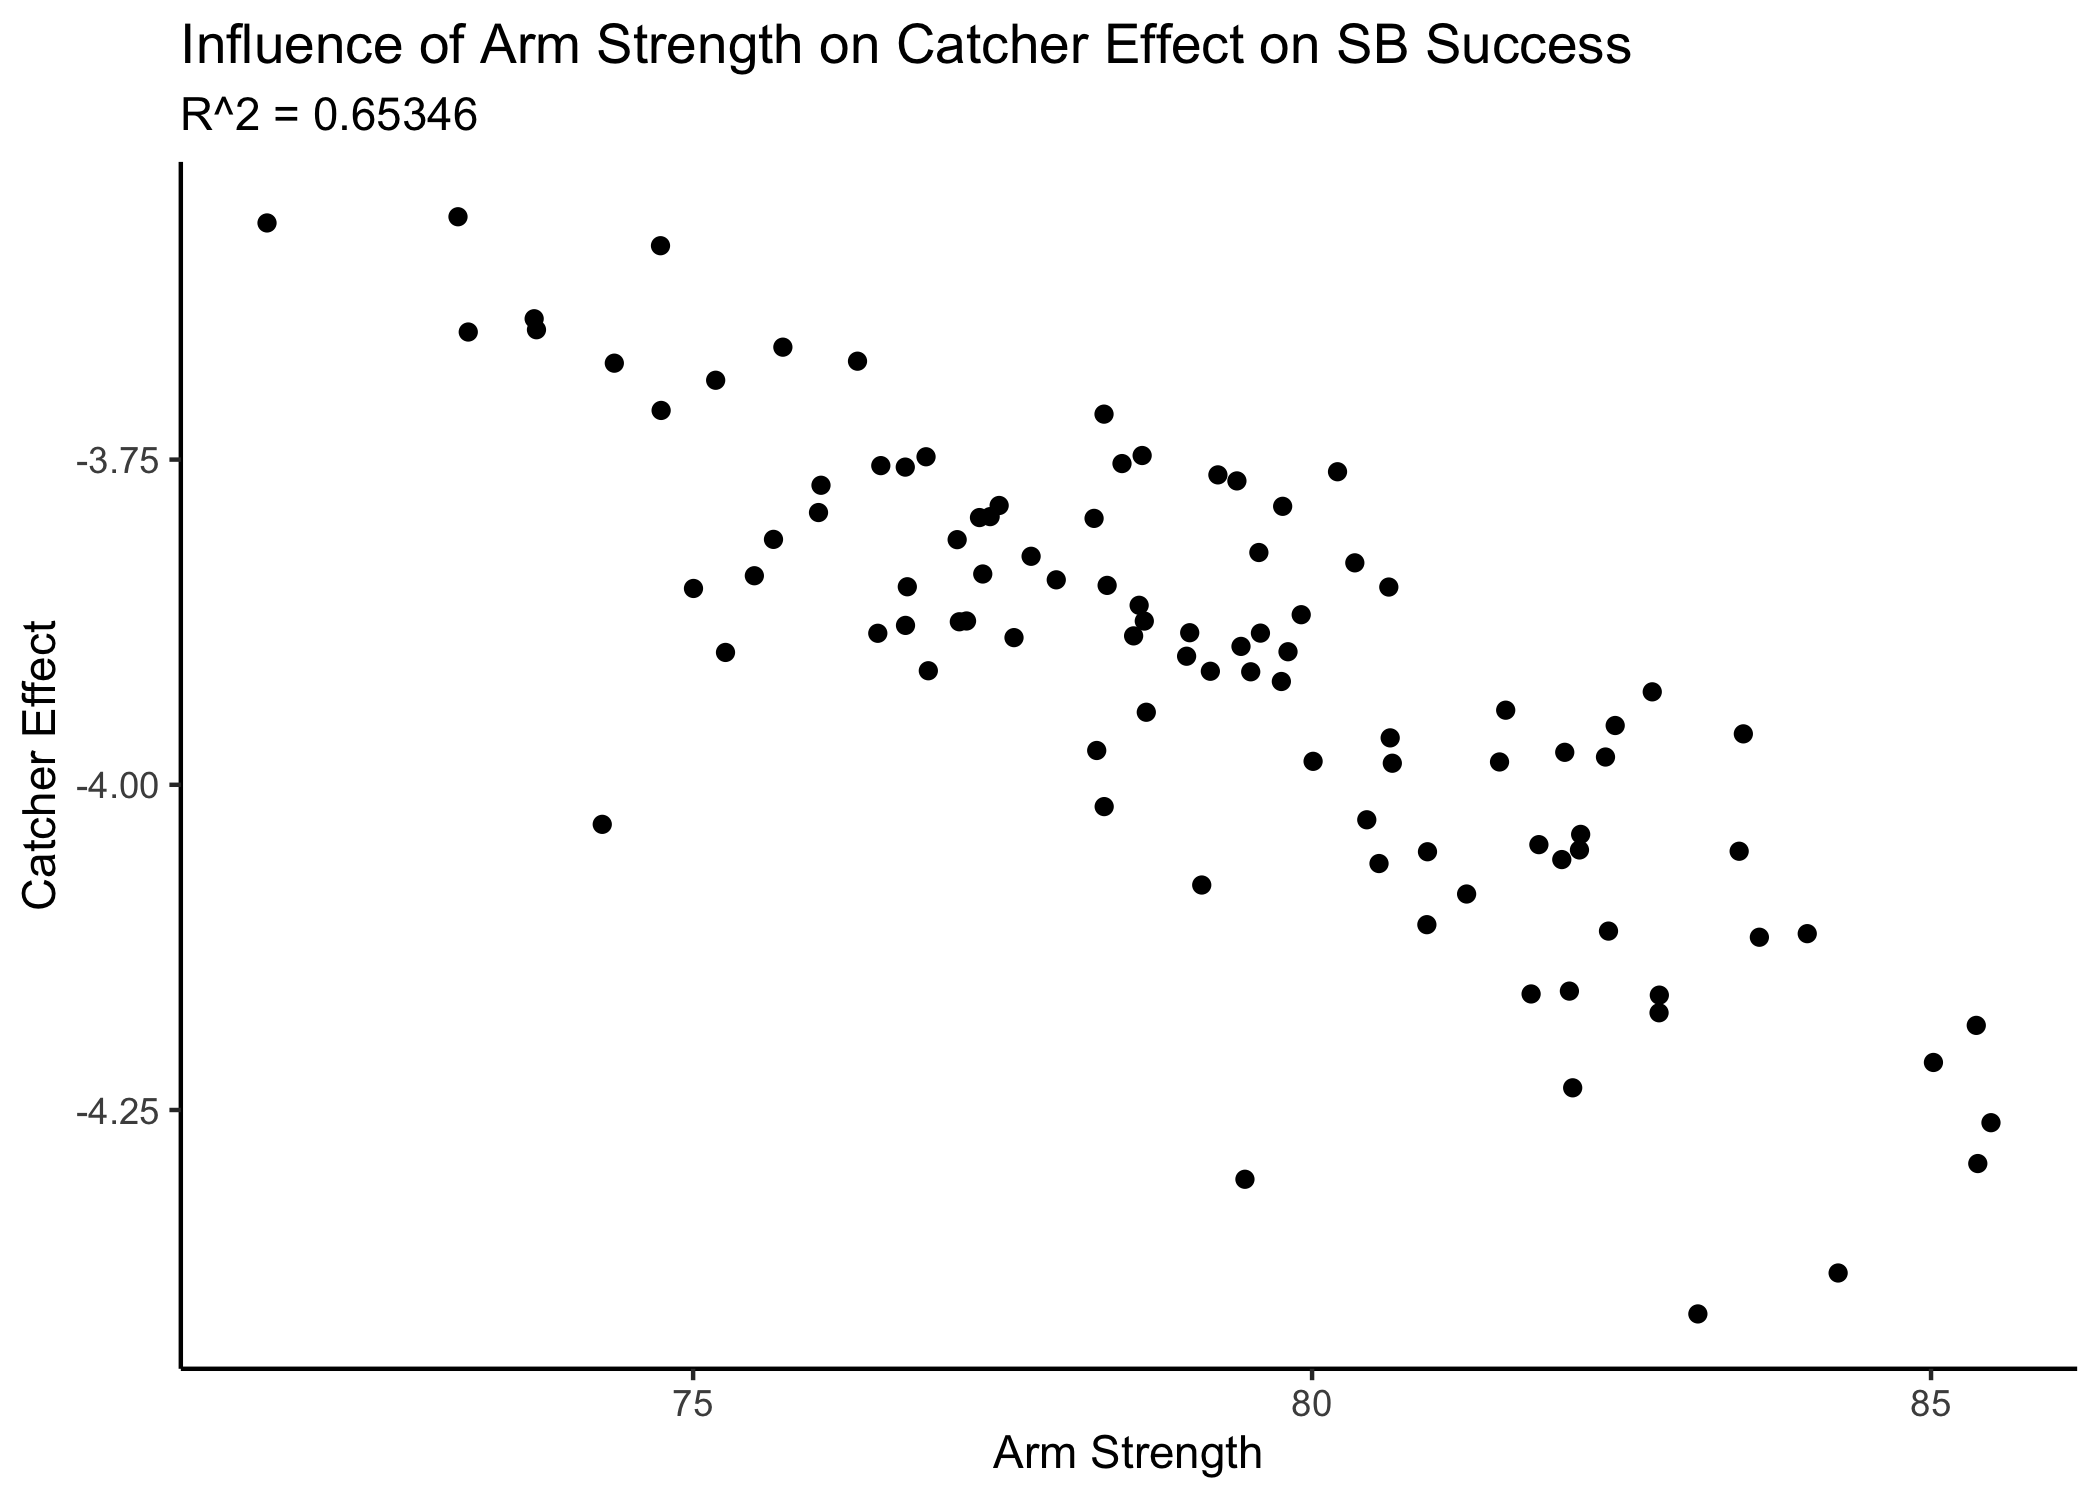
\includegraphics[width = 0.49\textwidth]{figures/catcher_effect.png}
        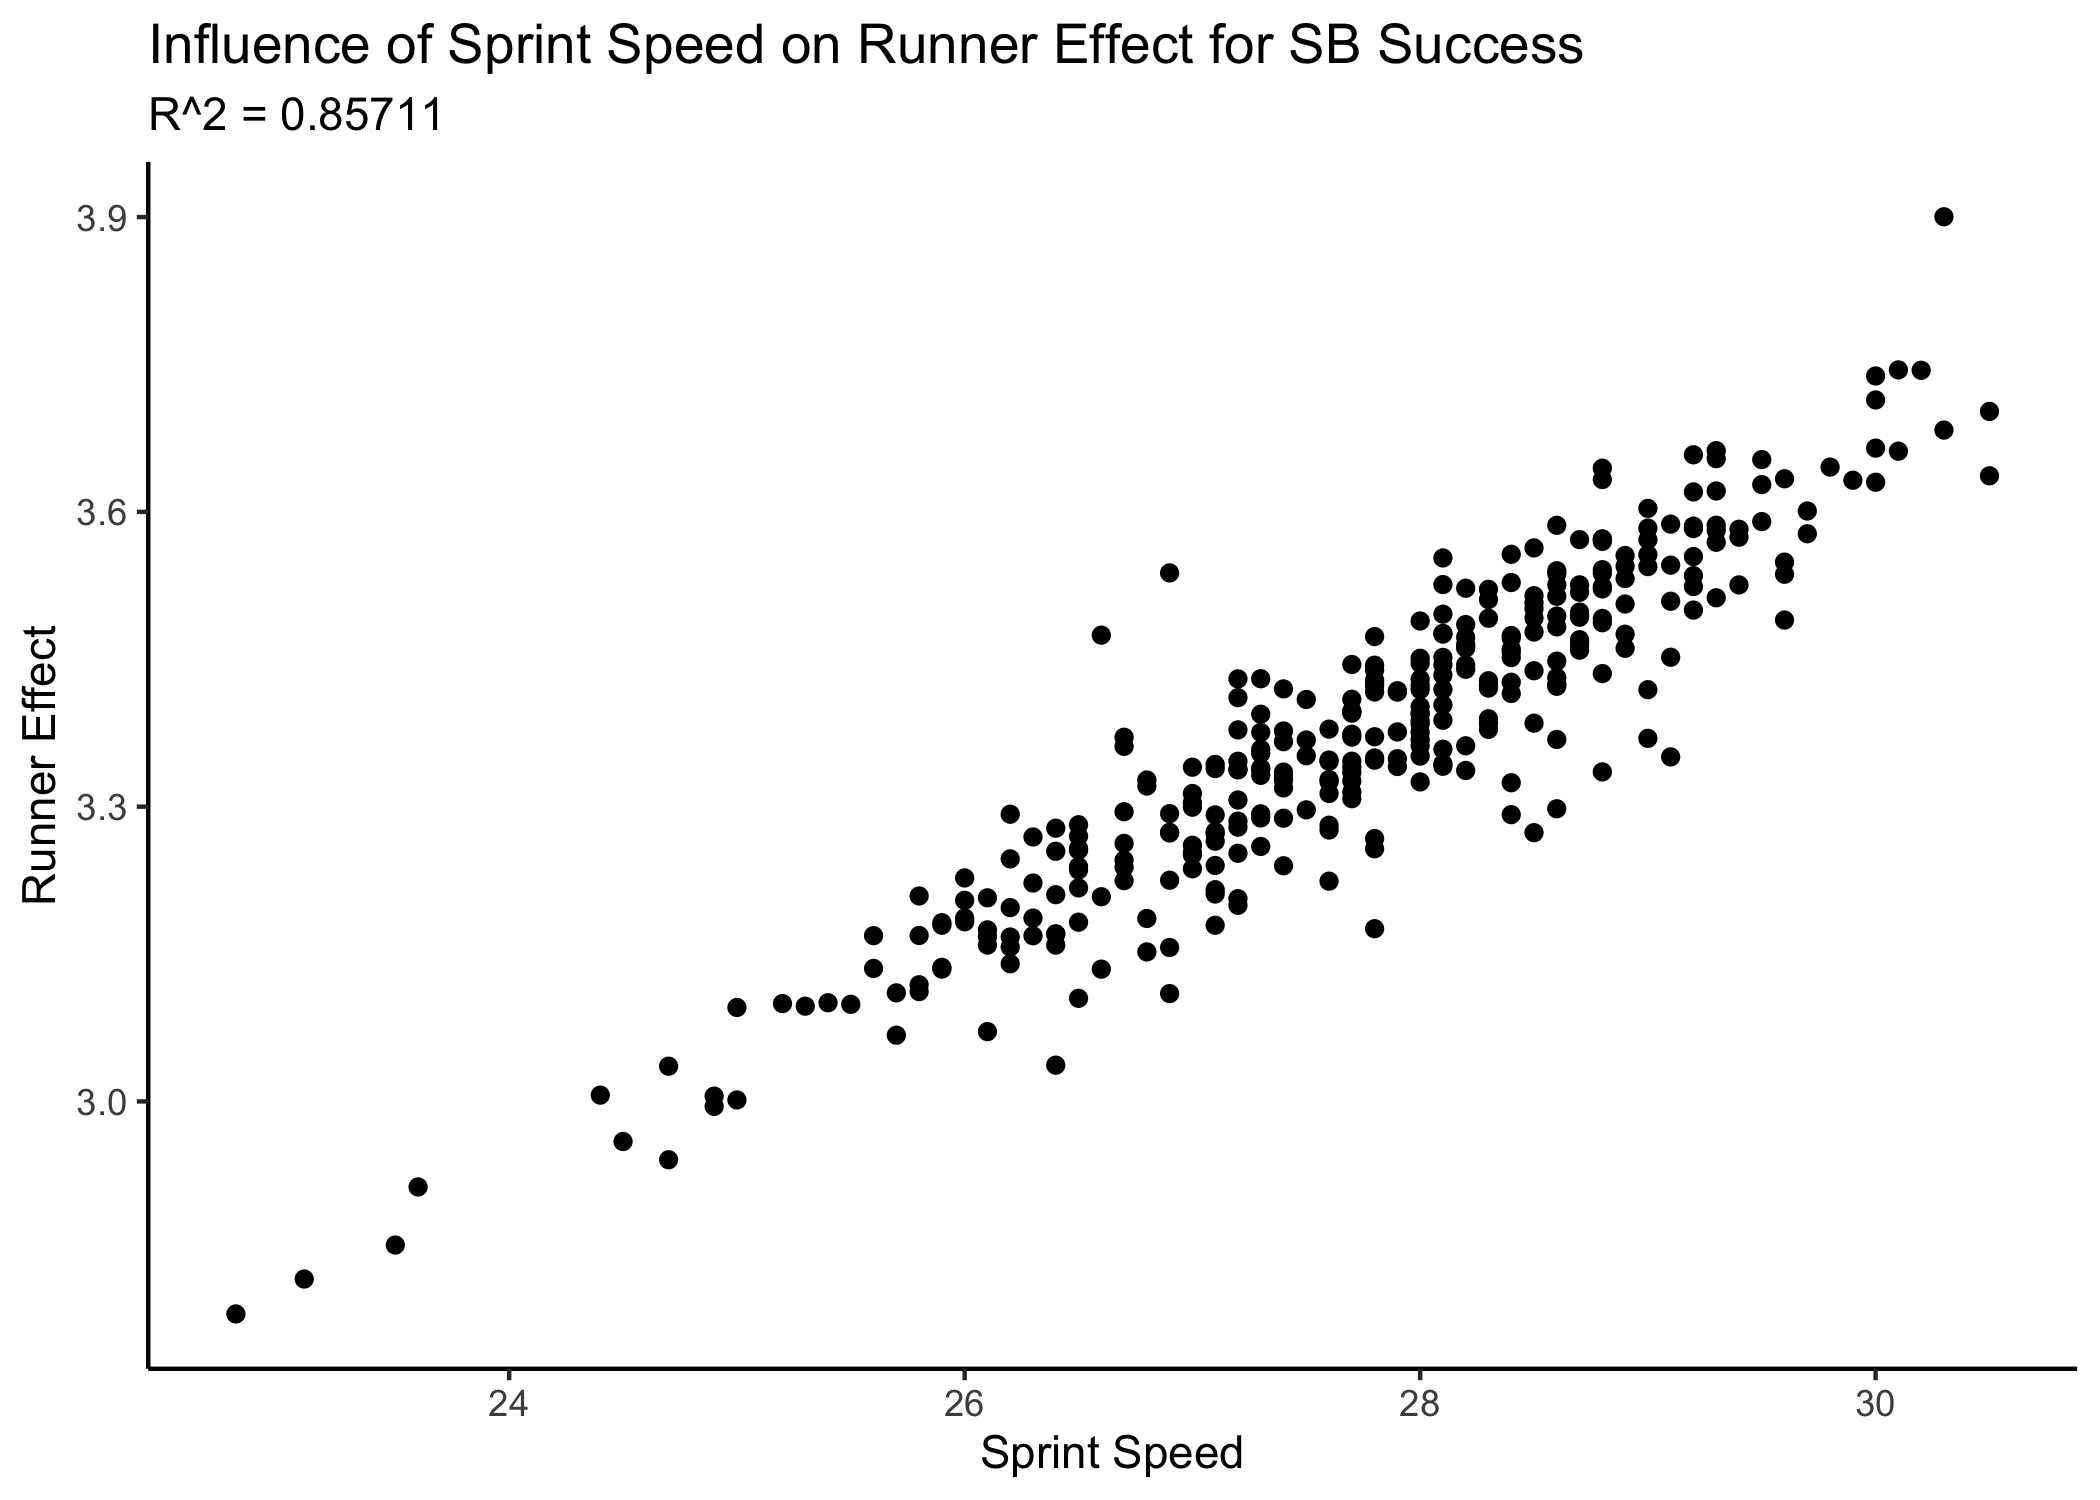
\includegraphics[width = 0.49\textwidth]{figures/runner_effect.png}
        \caption{
          \it
          (Left) The relationship between arm strength and catcher combined effect on stolen base success probability (relative to average, on the log-odds scale). The combined effect is the sum of the fixed effect due to arm strength and the catcher random effect.
          (Right) The relationship between sprint speed and runner combined effect on stolen base success probability (relative to average, on the log-odds scale). The combined effect is the sum of the fixed effect due to sprint speed and the runner random effect.
        }
        \label{fig:random-effect}
      \end{figure}

    \subsection{Single-agent Markov decision process}

      In the single-agent MDP, the only decision-maker is the runner, and they choose a policy for lead distance as a function of the game state, with the objective of maximizing the expected number of runs in the inning. In practice, the purpose of this MDP is to optimize runner decision-making given current conditions of pitcher behavior, anticipating that pitcher behavior will take some time to react to changes in runner behavior.

      Figure \ref{fig:finding-optimal-lead} illustrates how the runner would choose an optimal lead distance for different numbers of prior disengagements in an example scenario. Short lead distances have very low pickoff probabilities and low stolen base probabilities. As lead distance increases, stolen base probability increases, but so does pickoff probability. For very long lead distances, the run expectancy drops off sharply as the pickoff probability increases sharply. Between those two extremes, the runner strikes a balance to maximize run expectancy. The optimal lead distances for 0, 1 and 2 disengagements are 10.0 feet, 11.5 feet and 14.1 feet, respectively.
      
      \begin{figure}
        \centering
        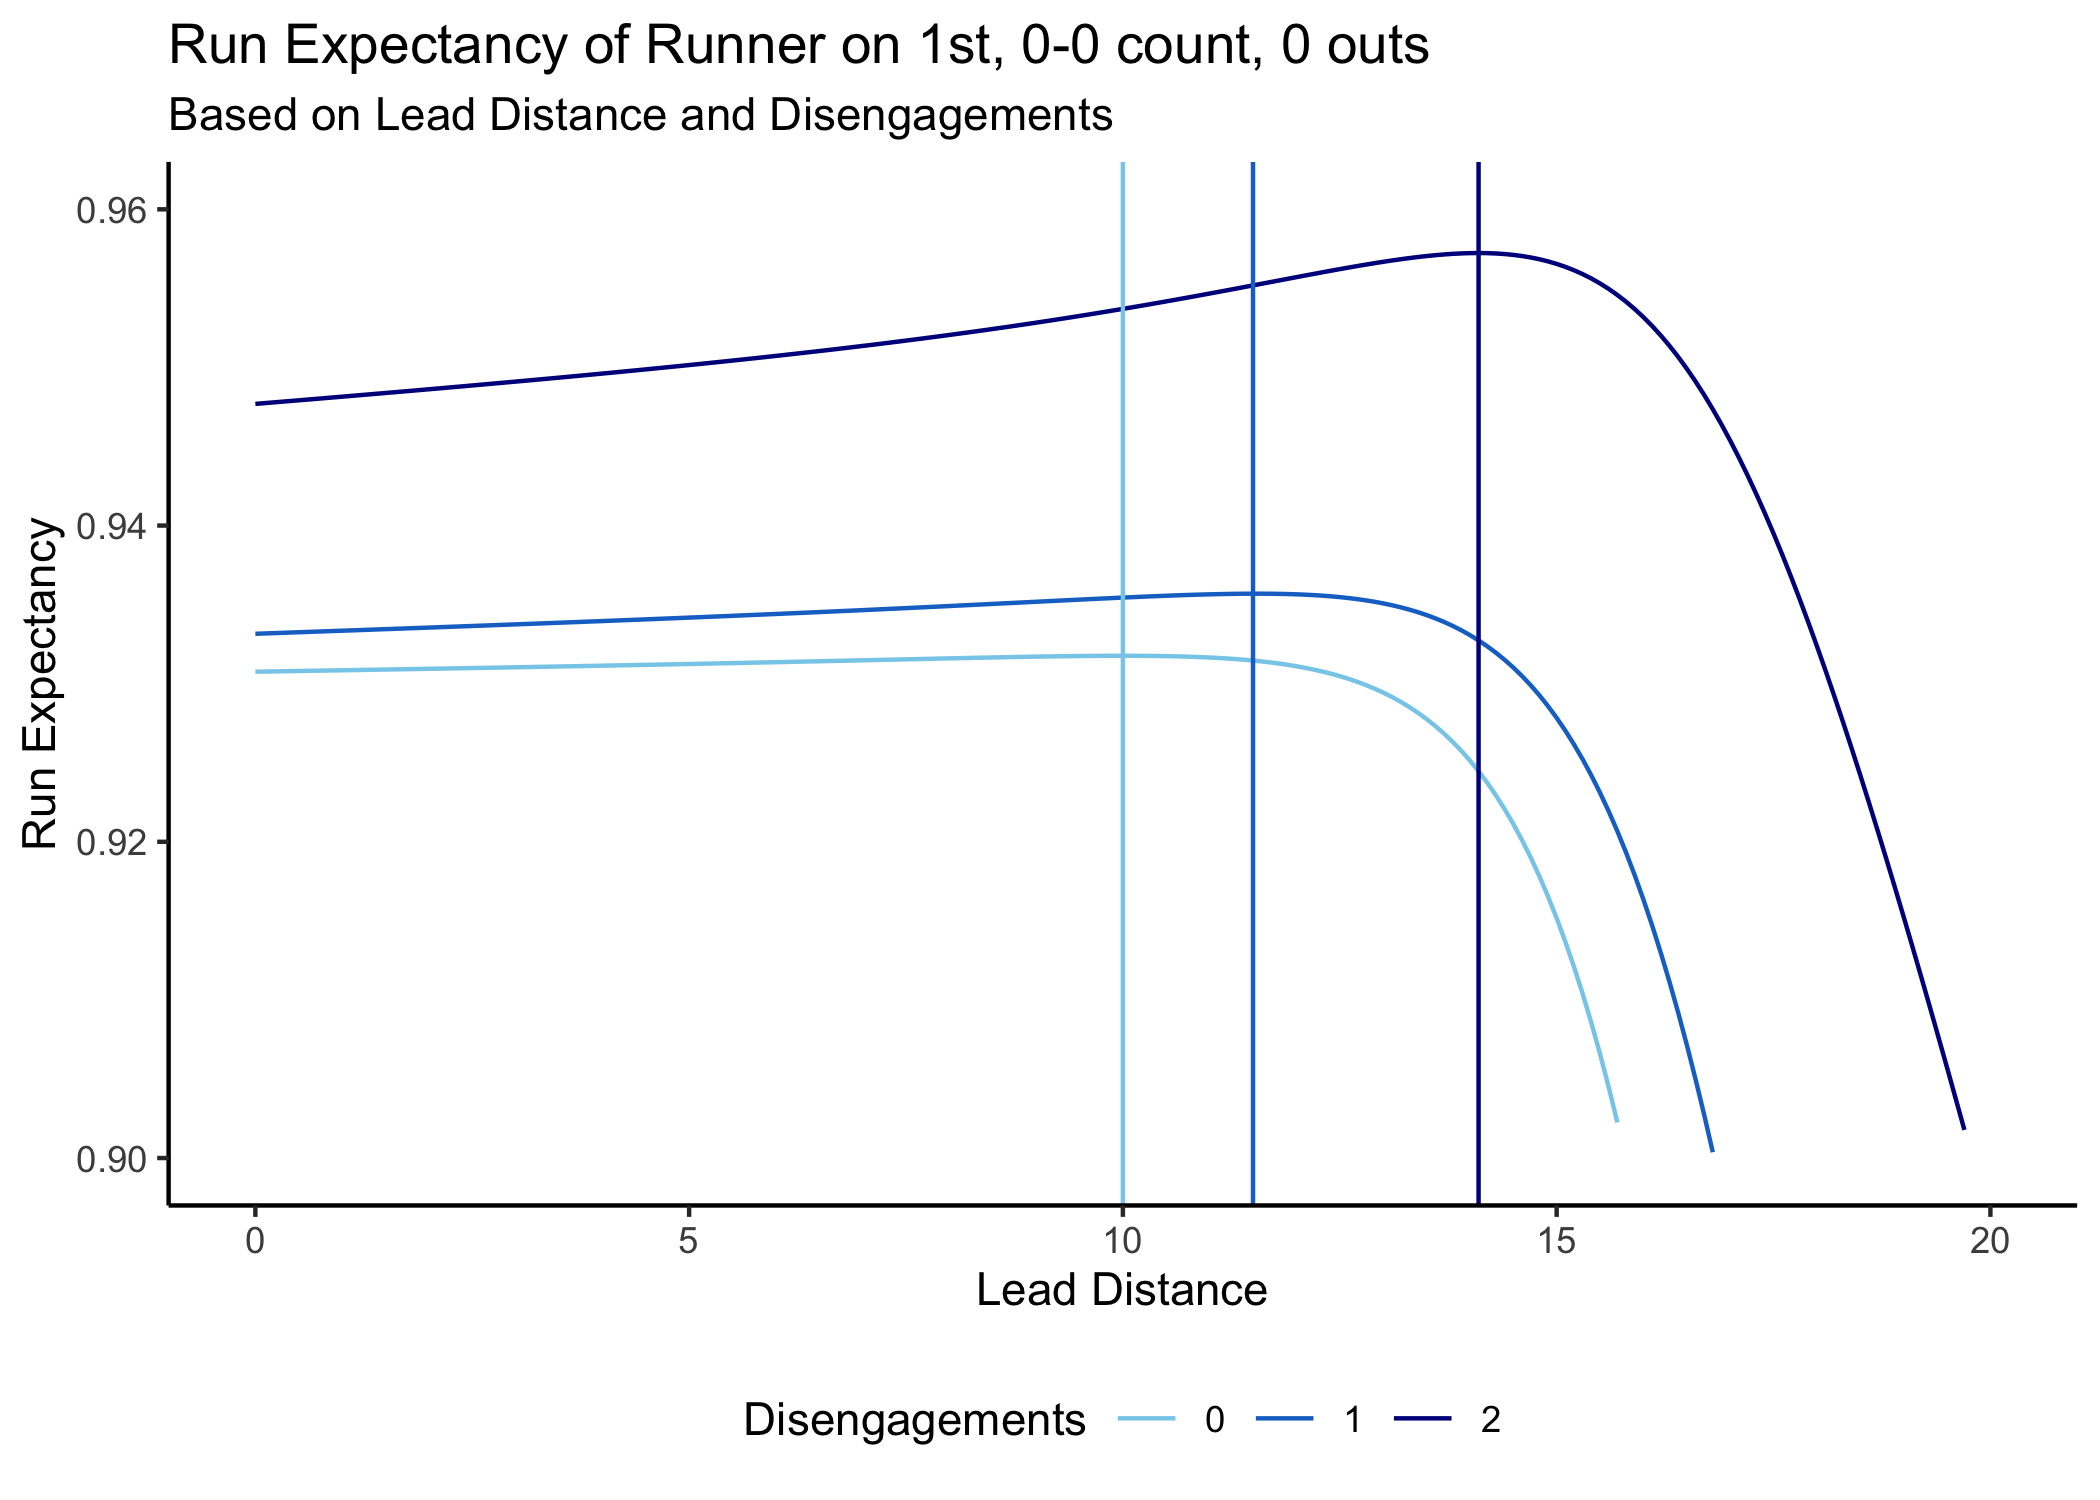
\includegraphics[width = 0.8\textwidth]{figures/finding_optimal_lead.png}
        \caption{
          \it Rest-of-inning run expectancy for different choices of lead distance. Three separate curves show the run expectancy for differing numbers of prior disengagements, assuming 0 balls; 0 strikes; 0 outs; third base unoccupied; and median player effects for pitcher, catcher and runner. Run expectancy is defined as the expectation of the value function $V_{\pi^*}$ (evaluated at the resulting state) corresponding to the optimal policy $\pi^*$ defined by (\ref{eqn:run-expectancy}). The vertical line corresponding to each curve marks the value at which the curve is maximized.
        }
        \label{fig:finding-optimal-lead}
      \end{figure}

      Policy iteration, as detailed by equations (\ref{eqn:update-value-single-agent}) and (\ref{eqn:update-policy-single-agent}), yields a policy $\pi^*$ optimizing rest-of-inning run expectancy. Tables \ref{tab:lead-by-count}, \ref{tab:lead-by-runners-outs} and \ref{tab:lead-by-players} report the optimal lead distance policy $\pi^*$ for different game states and player skills.
    
      Table \ref{tab:lead-by-count} shows how optimal lead distance varies by ball-strike count and number of prior disengagements, for an average runner facing an average battery (pitcher and catcher) with no outs. We observe that count has a mild influence on optimal lead distance, and lead distance has a strong influence. As the pitcher nears the disengagement limit, the runner has more incentive to extend their lead distance because pickoff attempts are less likely and a free base advancement (from a third unsuccessful pickoff attempt) is more likely.
 
      \begin{table}
        \centering
        \begin{tabular}{c|ccc}
          Count & \multicolumn{3}{c}{Disengagements}\\
                & 0 & 1 & 2\\
          \hline
          % latex table generated in R 4.3.1 by xtable 1.8-4 package
% Sun Jul 21 17:31:33 2024
 0-0 & 10.0 & 11.5 & 14.1 \\ 
  0-1 & 9.8 & 11.4 & 14.1 \\ 
  0-2 & 9.5 & 11.1 & 14.1 \\ 
  1-0 & 10.2 & 11.7 & 14.2 \\ 
  1-1 & 10.0 & 11.6 & 14.2 \\ 
  1-2 & 9.9 & 11.4 & 14.3 \\ 
  2-0 & 10.2 & 11.7 & 14.2 \\ 
  2-1 & 10.3 & 11.8 & 14.3 \\ 
  2-2 & 10.0 & 11.5 & 14.2 \\ 
  3-0 & 10.3 & 11.8 & 14.2 \\ 
  3-1 & 10.4 & 11.9 & 14.3 \\ 
  3-2 & 10.4 & 11.9 & 14.4 \\ 
  
        \end{tabular}
        \caption{
          \it The optimal lead distance policy (in feet) for an average runner facing an average battery (pitcher and catcher) with no outs.
        }
        \label{tab:lead-by-count}
      \end{table}
      
      Across counts, the recommended increase in lead distance is generally close to 1.5 feet after the first disengagement and 2.5 feet after the second disengagement. We observed this to be a good approximation across different runner/battery skills and different numbers of outs. Based on these results, we recommend the rule of thumb that runners increase their lead by two feet after each disengagement, a very simple and actionable guideline for athletes to follow.
    
      Table \ref{tab:lead-by-runners-outs} shows how optimal lead distance varies by number of outs, for an average runner facing an average batter with a 0-0 count, and Table \ref{tab:lead-by-players} shows how optimal lead distance varies by runner and battery skill, with 0 outs and a 0-0 count.

      \begin{table}
        \centering
        \begin{tabular}{c|ccc}
          Outs  & \multicolumn{3}{c}{Disengagements}\\
                & 0 & 1 & 2 \\
          \hline
          % latex table generated in R 4.3.1 by xtable 1.8-4 package
% Sun Jul 21 17:31:33 2024
 0 & 10.0 & 11.5 & 14.1 \\ 
  1 & 10.1 & 11.6 & 14.1 \\ 
  2 & 10.8 & 12.0 & 14.4 \\ 
  
        \end{tabular}
        \caption{
          \it Based on the number of outs in each row, each entry shows the optimal lead distance (in feet) for a runner on first depending on the number of disengagements.
        }
        \label{tab:lead-by-runners-outs}
      \end{table}

      Again, we see that each successive disengagement leads to an increase in recommended lead distance of approximately two feet. We also see that the recommended leads for 0 and 1 out are virtually identical, and are slightly longer with 2 outs. With 2 outs, stolen bases are more likely and pickoff attempts are less likely, so runners can be more aggressive.

    
      Table \ref{tab:players} shows the optimal lead distance for a runner on first base based on the players involved in the play. The runner skill level is based on sprint speed and their ability to steal bases. The battery skill level includes the pitcher and catcher's abilities to pick runners off and throw out potential basestealers, as well as the catcher's arm strength. This table assumes a 0-0 count, 0 outs, and nobody else on base:
    
      \begin{table}
        \centering
        \begin{tabular}{cc|ccc}
          Battery Skill  & Runner Skill & 0 Disengagements & 1 Disengagements & 2 Disengagements\\
          \hline
          % latex table generated in R 4.3.1 by xtable 1.8-4 package
% Sun Jul 21 17:31:33 2024
 10th Percentile Battery & 10th Percentile Runner & 10.5 & 11.9 & 14.5 \\ 
  10th Percentile Battery & Median Runner & 11.3 & 12.5 & 14.7 \\ 
  10th Percentile Battery & 90th Percentile Runner & 12.0 & 13.0 & 14.8 \\ 
  Median Battery & 10th Percentile Runner & 9.6 & 11.3 & 14.1 \\ 
  Median Battery & Median Runner & 10.3 & 11.7 & 14.1 \\ 
  Median Battery & 90th Percentile Runner & 11.0 & 12.1 & 14.2 \\ 
  90th Percentile Battery & 10th Percentile Runner & 7.8 & 9.8 & 12.6 \\ 
  90th Percentile Battery & Median Runner & 8.2 & 10.0 & 12.7 \\ 
  90th Percentile Battery & 90th Percentile Runner & 8.8 & 10.4 & 12.8 \\ 
  
        \end{tabular}
        \caption{
          \it Based on the skill of the battery (pitcher and catcher) and the skill of the runner in each row, each entry shows the optimal lead distance for a runner on first base depending on the number of disengagements.
        }
        \label{tab:lead-by-players}
      \end{table}

      The effect of the battery seems to be more significant than the effect of the runner. Facing a stronger pitcher and catcher cause the runner's optimal lead distance to shrink by several feet. We again see consistent results that runners should increase their lead by 1.5-2.5 feet upon each successive disengagement. However, better runners don't need to increase their leads by as much, likely because their stolen base success rates will be high to begin with.

      Currently, MLB runners are not doing a great job of putting pressure on the defense by maximizing their lead distances. Table \ref{tab:actual-vs-rec} compares the average actual and recommended leads for runners at 1st base with 2nd base open. With 0 disengagements, runners' actual leads come close to our recommendation, but they could often be adding an extra foot. As disengagements increase, we recommend about a 2 foot increase, but runners only tend to increase their leads by 0.6-0.7 feet. Runners overestimate the danger of a pickoff attempt under these situations, and could be increasing their team's run expectancy by adding a few feet to their lead distances here. Runners rarely meet or exceed the lead distance we recommend, especially with 1 or 2 disengagements.

      \begin{table}
        \centering
        \begin{tabular}{c|ccc}
          Disengagements & Average Actual Lead & Average Recommended Lead & Actual Exceeds Recommendation\\
          \hline
          % latex table generated in R 4.3.1 by xtable 1.8-4 package
% Sun Jul 21 20:01:27 2024
 0 & 9.5 & 10.4 & 28.9\% \\ 
  1 & 10.2 & 11.8 & 10.4\% \\ 
  2 & 10.8 & 14.4 & 0.7\% \\ 
  
        \end{tabular}
        \caption{
          \it Each entry shows the average lead at 1st base based on the number of disengagements prior to the pitch. The recommended leads in the final column are based on our single-agent model. The final column shows the percent of pitches where the actual lead exceeds our recommendation.
        }
        \label{tab:actual-vs-rec}
      \end{table}

      In order to quantify the effect of optimizing baserunners' lead distances, we compared the run expectancy at the start of an inning before and after iterating through the Bellman Equation. In the 2023 season, the run expectancy of an inning was 0.5163 runs. After our policy iteration, the run expectancy jumped to 0.5277 runs. This increase of 0.0114 runs per inning may seem very small, but this difference adds up quickly. Over a 162 game season, adding 0.0114 runs per inning increases a team's run total by 16.68 runs. Using the typical valuation of \$1 Million per run, optimizing baserunners' lead distances could be worth nearly \$17 Million to a team under the current conditions. This is an incredibly valuable result that does not require much effort for a team to implement.

    \subsection{Two-agent Markov decision process}

      All of the results shown so far correspond to our single-actor model, where a runner choose a lead distance and all other outcomes are probabilistic based on their choice. Now, we expand our model to a two-actor model, where the runner first chooses a lead distance, then the pitcher elects whether to attempt a pickoff or throw a pitch. The pitcher makes whichever decision minimizes the run expectancy for the offensive team. Therefore, in order for the runner to maximize their run expectancy, they should choose a lead distance such that the pitcher is indifferent as to whether to attempt a pickoff or throw a pitch. Pitchers should always attempt a pickoff if the runner's lead extends beyond this distance, and should always throw a pitch if the lead is shorter. This is the game theoretic equilibrium.

      Table \ref{tab:count-twoagent} shows the optimal lead by count under the two-agent model:

      \begin{table}
        \centering
        \begin{tabular}{c|ccc}
          Count & 0 Disengagements & 1 Disengagement & 2 Disengagements\\
          \hline
          % latex table generated in R 4.3.1 by xtable 1.8-4 package
% Sun Jul 21 17:35:38 2024
 0-0 & 11.2 & 11.8 & 16.2 \\ 
  0-1 & 10.8 & 11.3 & 16.2 \\ 
  0-2 & 10.2 & 10.8 & 16.2 \\ 
  1-0 & 11.2 & 12.0 & 16.1 \\ 
  1-1 & 10.9 & 11.1 & 16.1 \\ 
  1-2 & 10.5 & 10.4 & 16.3 \\ 
  2-0 & 11.0 & 12.2 & 15.9 \\ 
  2-1 & 11.0 & 12.1 & 15.9 \\ 
  2-2 & 10.4 & 11.4 & 15.9 \\ 
  3-0 & 10.4 & 11.6 & 15.3 \\ 
  3-1 & 10.5 & 11.6 & 15.7 \\ 
  3-2 & 10.3 & 11.1 & 15.6 \\ 
  
        \end{tabular}
        \caption{
          \it Based on the count in each row, each entry shows the optimal lead distance (in feet) for a runner on 1B depending on the number of disengagements for our two-agent model.
        }
        \label{tab:count-twoagent}
      \end{table}

      Under this game-theoretic equilibrium, we see that runners should be taking even longer leads in most situations. This is likely because pickoffs are often wasteful at lower lead distances. If pitchers were to optimize their pickoff behavior, then runners would be able to get longer leads before a pickoff becomes worthwhile for the pitcher. Our two-foot rule of thumb from the single-agent model doesn't hold here. Instead, we see a recommended increase of about 0.5-1 feet after 1 disengagement, and a recommended increase of around 3.5-5 feet after the 2nd disengagement. Once a pitcher reaches 2 disengagements, it becomes extremely risky to attempt a pickoff, so runners can take advantage of that by extending their leads beyond 15 feet.

      In order to evaluate how well pitchers follow our recommendations, we looked back at all situations from the 2023 season with a runner on first base only. Our two-agent model suggests that pitchers should have attempted a pickoff in 8.3\% of these situations. In reality, they only attempted pickoffs 5.6\% of the time.

      In situations where our model suggested a pickoff, pitchers actually attempted a pickoff 10.8\% of the time in 2023.

      In situations where our model suggests throwing a pitch, pitchers actually attempted a pickoff 5.0\% of the time.

      Overall, it seems that pitchers should be attempting more pickoffs. If runners start increasing their lead distances in the way we recommend, then pitchers should respond by picking off even more often.

      Under this equilibrium of optimal pitcher and baserunner behavior, runners still hold a slight advantage compared to the status quo, but not by much. We calculated that runners could increase their team's run expectancy by about 0.0036 runs per inning by following these lead recommendations if pitchers also optimized their behavior. Over a 162 game season, this adds up to 5.2 runs. Ultimately, the current behavior of pitchers and runners is not far from the Nash Equilibrium. However, both sides could improve their team's performance by several runs by optimizing their behavior surrounding the running game.

  \section{Discussion}

  \section{Assumptions}

    \begin{itemize}
      \item NOTE (SP): Let's try including pitcher handedness in our model
      \item NOTE (SP): Should we use catcher pop time instead of arm strength?
      \item Successful pickoff eliminates runner with no other runner movement
      \item Number of disengagements does not affect batter outcomes
      \item Lead distance does not affect outcomes on batted balls (note: domain knowledge tells us that secondary lead is more important than the lead distance we observe, which is first pitcher movement)
      \item We are ignoring the possibility that the runner takes off for 2B on a pickoff attempt
      \item Other than pickoff attempts, no other disengagements occur
    \end{itemize}

  \section{Acknowledgments}

    Major League Baseball trademarks and copyrights are used with permission of MLB Advanced Media, L.P. All rights reserved.

  \bibliography{arxiv}

\end{document}
